\chapter{Simulations}
\label{simulations}

In order to test and validate the different algorithms from chapter \ref{algos}, a simulation was implemented. The advantages of such simulations is to get rid of the technical compulsions of electronic materials, no configuration of the antennas was needed, no need to implement features in the application to deal with the \gls{cir}, no need to modify the state machines presented in appendix \ref{app:state_machine}, etc.
\vspace{2mm}

However, this simulation needs to be as true as possible compared with the reality. This implementation is detailed in the first section of this chapter. Then, the results obtained using this simulation are developed in the following sections for the locating methods in \ref{algos}.

\section{Simulation}

The simulation has been created by adapting a previously developed code for the project of the course of Communication Channel given at the ULB \cite{dedoncker2019course}. This simulation is based on the ray tracing, a technique used to compute the route of electro-magnetic waves detailed in section \ref{ray_tracing}. Two important features of this program can be separated. The first objective being to simulate a realistic \gls{cir} similar to the one produced by the experimental set-up. The second is to perform the localization based on this realistic \gls{cir}.
\vspace{2mm}

\subsection{Realistic CIR generation}

To reach this purpose, first the wished environment has to be simulated in the program. To make it happen, the $\texttt{room\_configuration.m}$ file has been created. Configuration of the geometry of the room, the type of walls used, the number of different furniture and their location in the room can also be chosen. This file is also used to choose the location of the anchor and the tag in the room. The left figure of the Fig. \ref{fig:peaks_real} has been produced using this configuration file.
\vspace{2mm}

In order to generate a finite-band \gls{cir}, the equivalent infinite-band \gls{cir} is first generated. This can be done for a direct ray, simple reflected ray, double reflected ray and triple reflected ray the transmission across the different materials is also taken into account. The ray reflected on the ground is also computed but not shown for the sake of clarity. An example of all the other ray can be found in Fig. \ref{fig:ray_simu}. On this figure, furniture are displayed against the walls, the direct ray is displayed in red, a simple reflected ray on one of the furniture in blue, a double reflected ray in cyan and a triple reflection ray is displayed in green.

\begin{figure}[H]
\centering
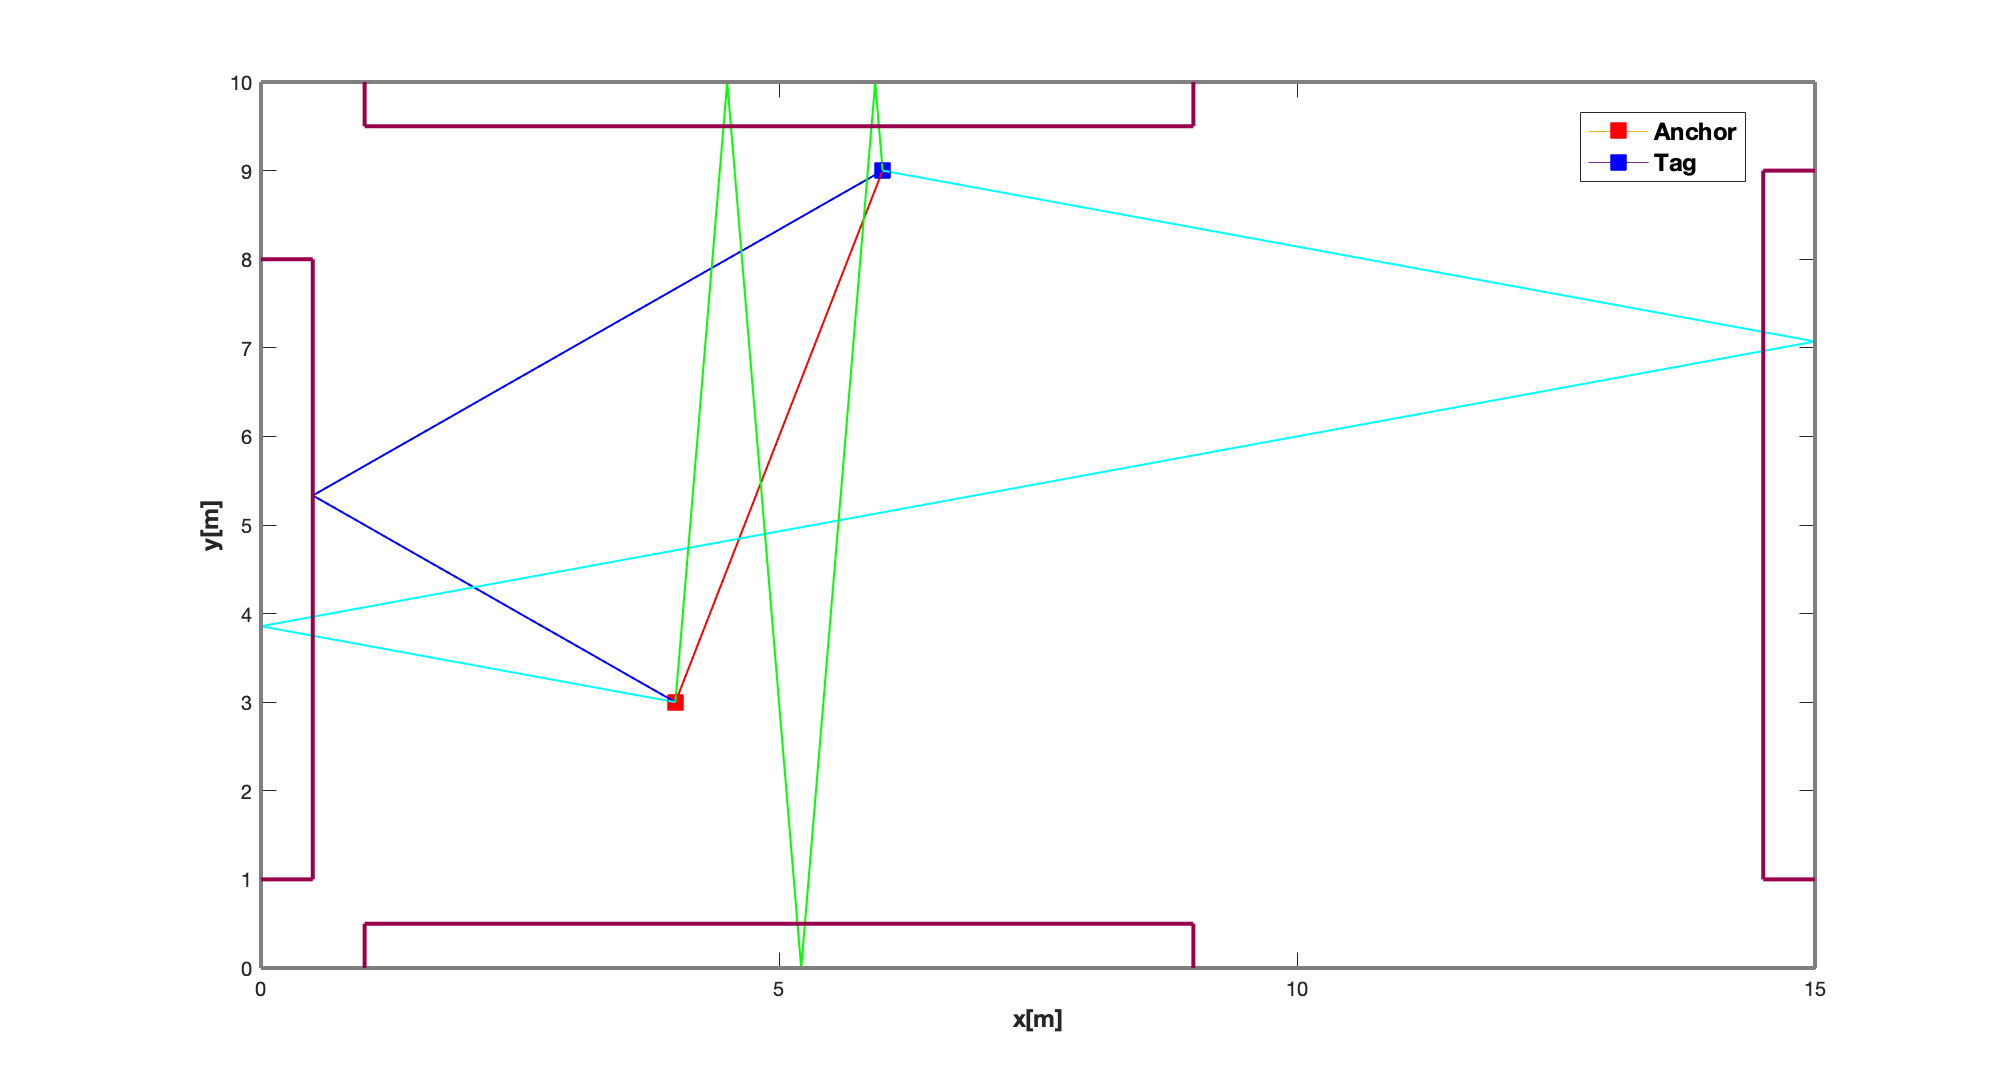
\includegraphics[width=.75\linewidth]{Images/rays_example.png}
\caption{Ray Tracing Simulation - Example. \label{fig:ray_simu}}
\end{figure}

Stating infinite is not completely correct, the real bandwidth being that of the carrier frequency in this case, however, it shows the characteristics in connection with actual bandwidth used. The different peaks are well isolated and punctual. The so-called infinite-band \gls{cir} is converted into the frequency domain using the Fourier transform. The built-in \gls{fft} function from $\text{MATLAB}$ has been used \cite{mathworks}. The frequency spectrum has been reduced from the carrier frequency to $\text{500 MHz}$, an approximation of the bandwidth used as detailed in section \ref{dwm1000}. Using the \gls{ifft} to go back into the time domain results in the red curve on Fig. \ref{fig:conv_fin}.

\begin{figure}[H]
\centering
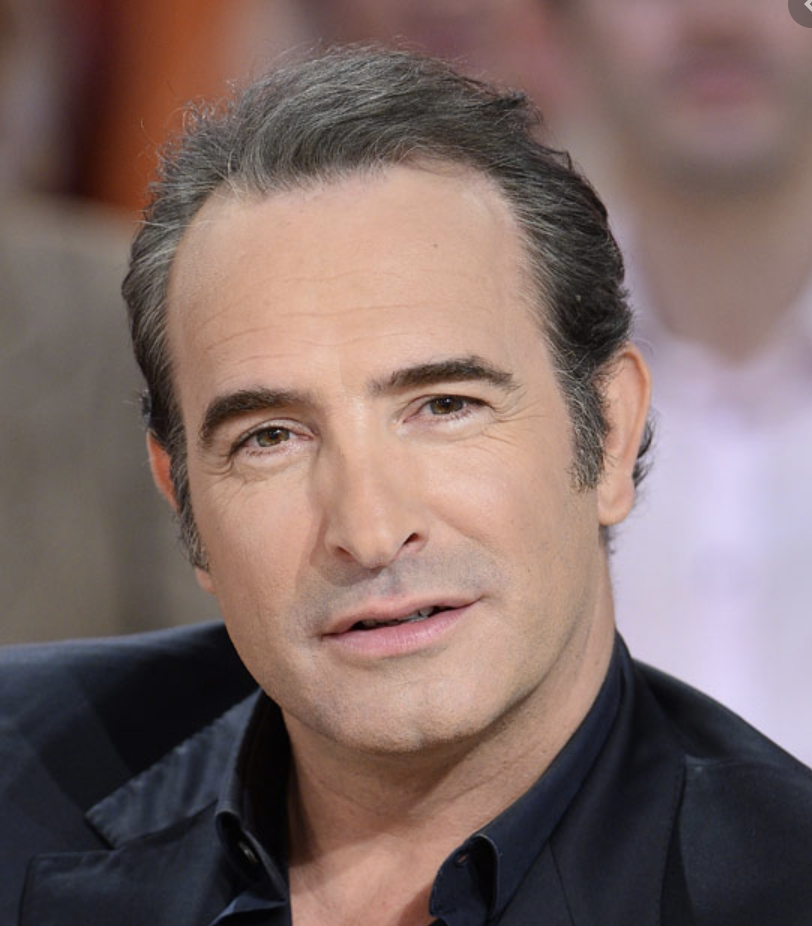
\includegraphics[width=.2\linewidth]{Images/Temporary_pic.png}
\caption{Trouver un nom \label{fig:conv_fin}}
\end{figure}

As we can observe, this \gls{cir} is far from ideal, mostly because of the sides lobes appearing near to every peak. This is a side effect because of the reduction of the bandwidth. In order to counteract this effect, a Chebyshev window has been used \cite{lynch1997dolph}, \cite{mathworks}. The convolution of the finite-band time domain \gls{cir} will reduce those side lobes. The orange curve from Fig. \ref{fig:conv_fin} has been produced using the $\text{chebyshev}$ function from MATLAB. The parameter of the Chebyshev window has been set heuristically to 25. A systematic method would have to use an experimental and a simulated \gls{cir} that would correspond to the same situation\footnote{The same room, antennas configuration, antennas position, ...}. The optimal parameter would then be computed using the $\text{lsqcurvefit}$ function from MATLAB.

\subsection{Analysis tools}

To evaluate the quality of the localization, several tools have been developed to give some visual clues to assess the performance of such algorithm and analyze the origin of those results. Those tools can be split into two categories.
\vspace{2mm}

The \gls{sla}, for each anchor - tag configuration in a specific room, \gls{cir} can be generated with the extracted peaks shown on the same figure. Those \gls{cir} are configurable based on the number of reflections which is wanted. A \gls{mse} map can also be generated, which will actually be the value $S(\vec{p_0})$ for each possible location\footnote{In the restricted solution space.} of the tag for a specific tag - anchor combination. About, the \gls{hla} also provides the wished \gls{cir} with its associate peaks recuperated. Since we are solving a system, all the computed solutions of the system for each combination of \glspl{va} can be accessed. 
\vspace{2mm}

Both method finally provide a map displaying, for each tag location, the error distance between the estimated tag location and its exact location for a given anchor. Allowing to visually assess the success rate of setting an anchor at some specific coordinates.

\section{Soft Simulation}
\label{soft_sim}

This section allows us to see some results obtained using the \gls{sla} in order to characterize the best places to put an anchor and evaluate the possibilities of such algorithms. First, the symmetry issue is discussed, giving some primary clues made about the location of such an anchor. Second and third, more complex cases are investigated using room filled with furniture, several anchor locations being discussed.

\subsection{Symmetry issues}
\label{sym_cases}
\begin{figure}[H]
\centering
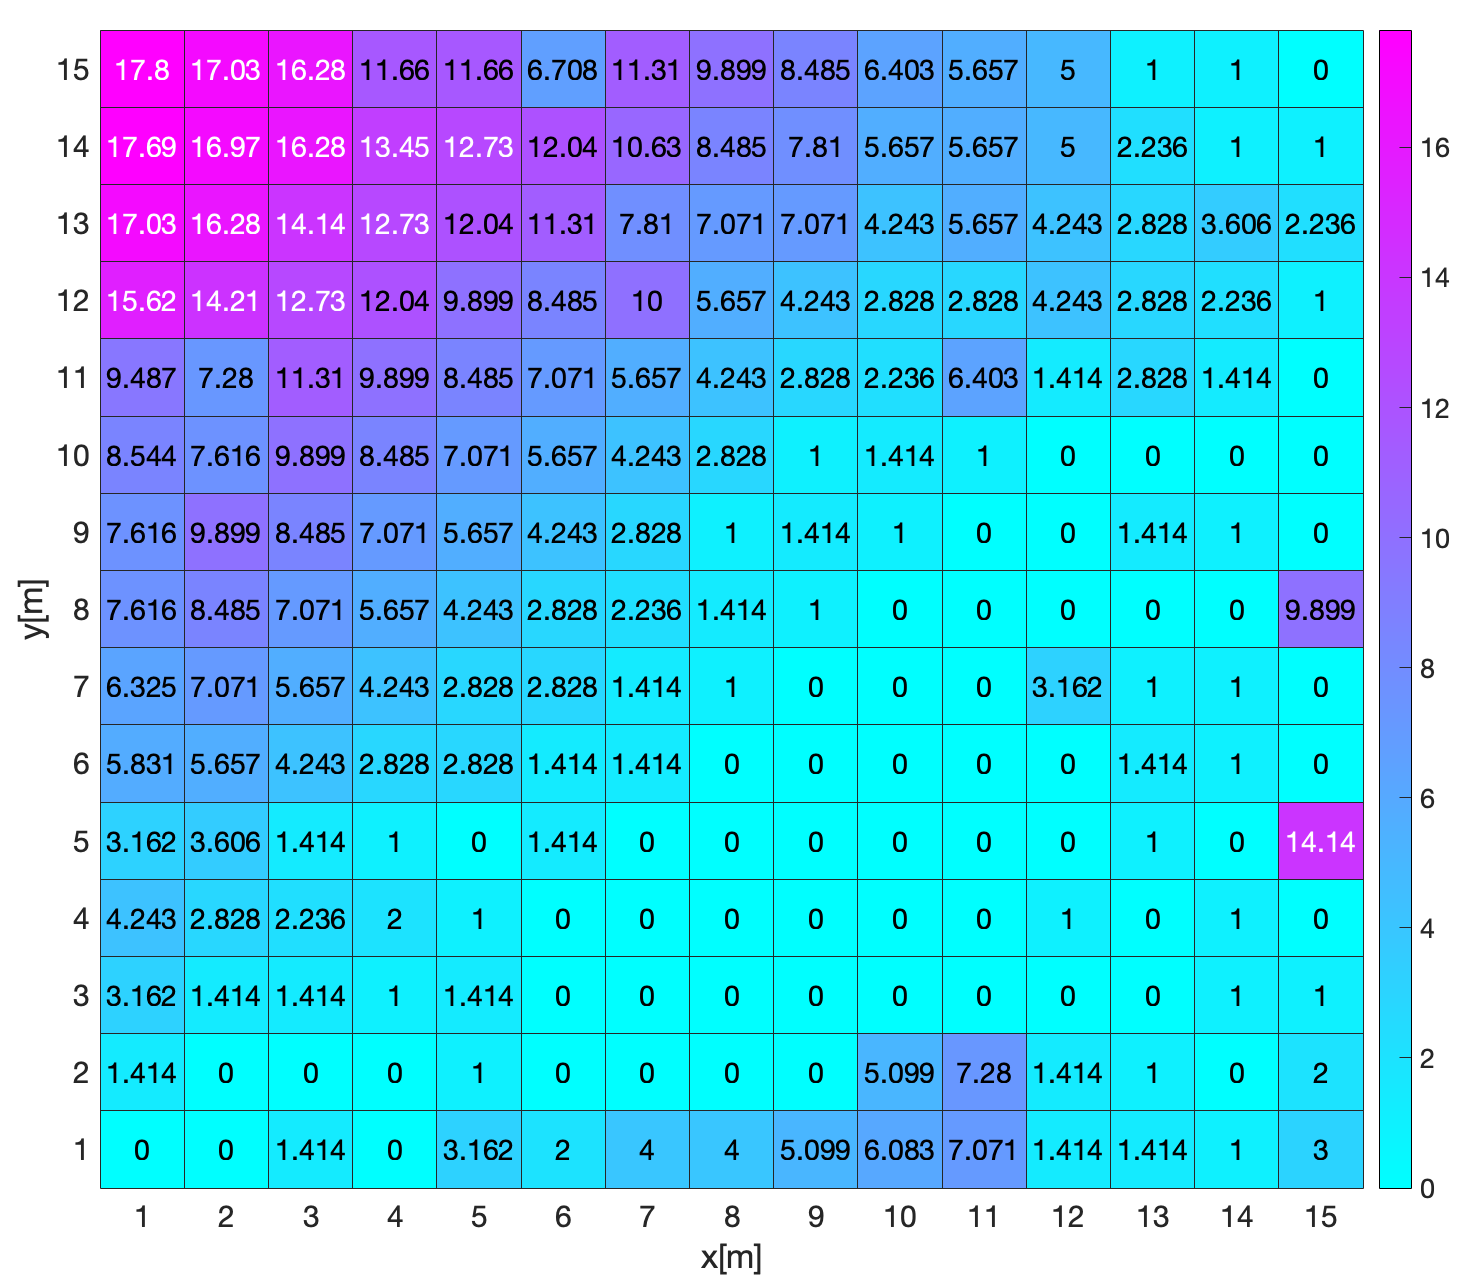
\includegraphics[width=.73\linewidth]{Images/15_15_sym.png}
\caption{Distance [m] between the tag exact location and the estimation provided by the \gls{sla}. Empty room of 15 by 15 meters, anchor set in (2, 2). Five peaks extracted from the CIR. \label{fig:square_sym}}
\end{figure}

An issue occurring with the 'one anchor' localization paradigm highlighted in section \ref{hard_loc} is the symmetry. This issue was discussed in the case of hard localization because of the axial symmetry between \glspl{va}, leading to mingled paths on the \gls{cir}. Another kind of symmetry issue can be seen on Fig. \ref{fig:square_sym}, approximatively half of the locations of the tag was correctly estimated.
\vspace{2mm}

Because of the location of the anchor, a symmetry appears in this room, the axial symmetry being the diagonal starting at the bottom left until the top right of the Fig. \ref{fig:square_sym}. This is confirmed by Fig. \ref{fig:square_sym_cir_comparison}. The \gls{mse} for each possible location in the solution space generated by the space solution reduction algorithm is shown. We can observe the symmetry across the bottom-left to top-right diagonal. This symmetry is not completely perfect, some location gets a small location error as (5, 2), which wrongly estimates the location by 1 meter, the origin of such particular cases is studied in section \ref{soft_empty_room}.

\begin{figure}[H]
\centering
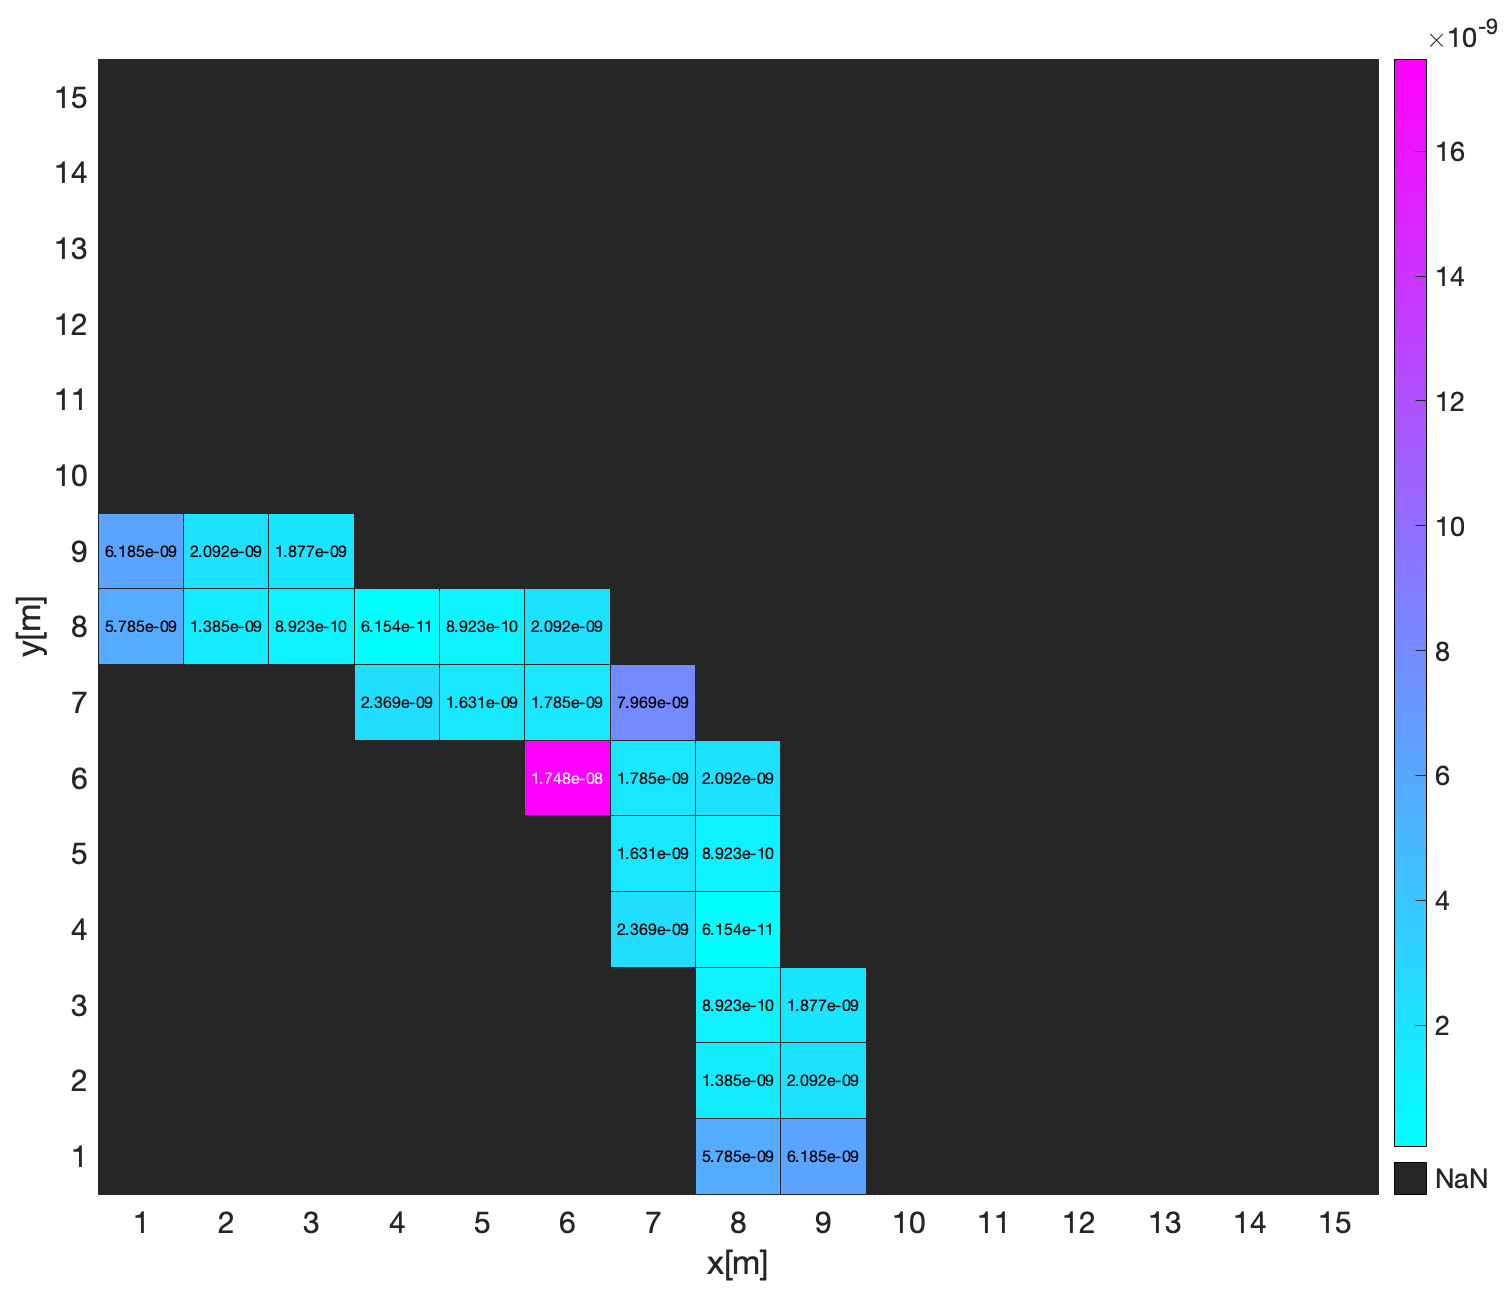
\includegraphics[width=.9\linewidth]{Images/square_sym_mse_4_8.png}
\caption{MSE map generated with an anchor in (2, 2) and the tag being located at (8, 4). The room configuration is an empty rectangle of 15 by 10 m.  \label{fig:square_sym_cir_comparison}}
\end{figure} 

To avoid such errors, we should avoid placing the anchor in such a symmetric position. We can even generalize this result by stating that we should avoid setting the anchor on any axis of symmetry of the room, being the diagonals and the medians in a square. Such cases are shown in appendix \ref{app:symmetry_antenna_placement}, where the anchor has been set on a axis of symmetry.
\vspace{2mm}

We could assume that this issue only occurs in square and not in rectangular rooms. Indeed, the diagonals of a rectangle are not part of its axis of symmetry, only its medians are. If those anchors are not on an axis of symmetry, there is no reason to obtain systematically twice the same \gls{cir}. Therefore, we could think that by avoiding those axis, this symmetry issue would also be avoided.
\vspace{2mm}

However, as it is shown on Fig. \ref{fig:rect_sym}, part of the \gls{cir} generated for (4, 8) and (8, 4) are the same when the anchor is set at (2, 2). The three extracted peaks, corresponding to the direct ray and the reflected rays only once on the bottom and left walls, are equivalent, the beginning of the \gls{cir} being mostly identical in both cases. We can conclude that the number of peaks extracted is an important parameter of this locating system. If too few peaks are taken, it may be impossible to distinguish several cases. If too many are taken, some irrelevant peaks could be extracted from the realistic \gls{cir}. This being noisier because of the different reflections happening.

\begin{figure}[H]
\centering
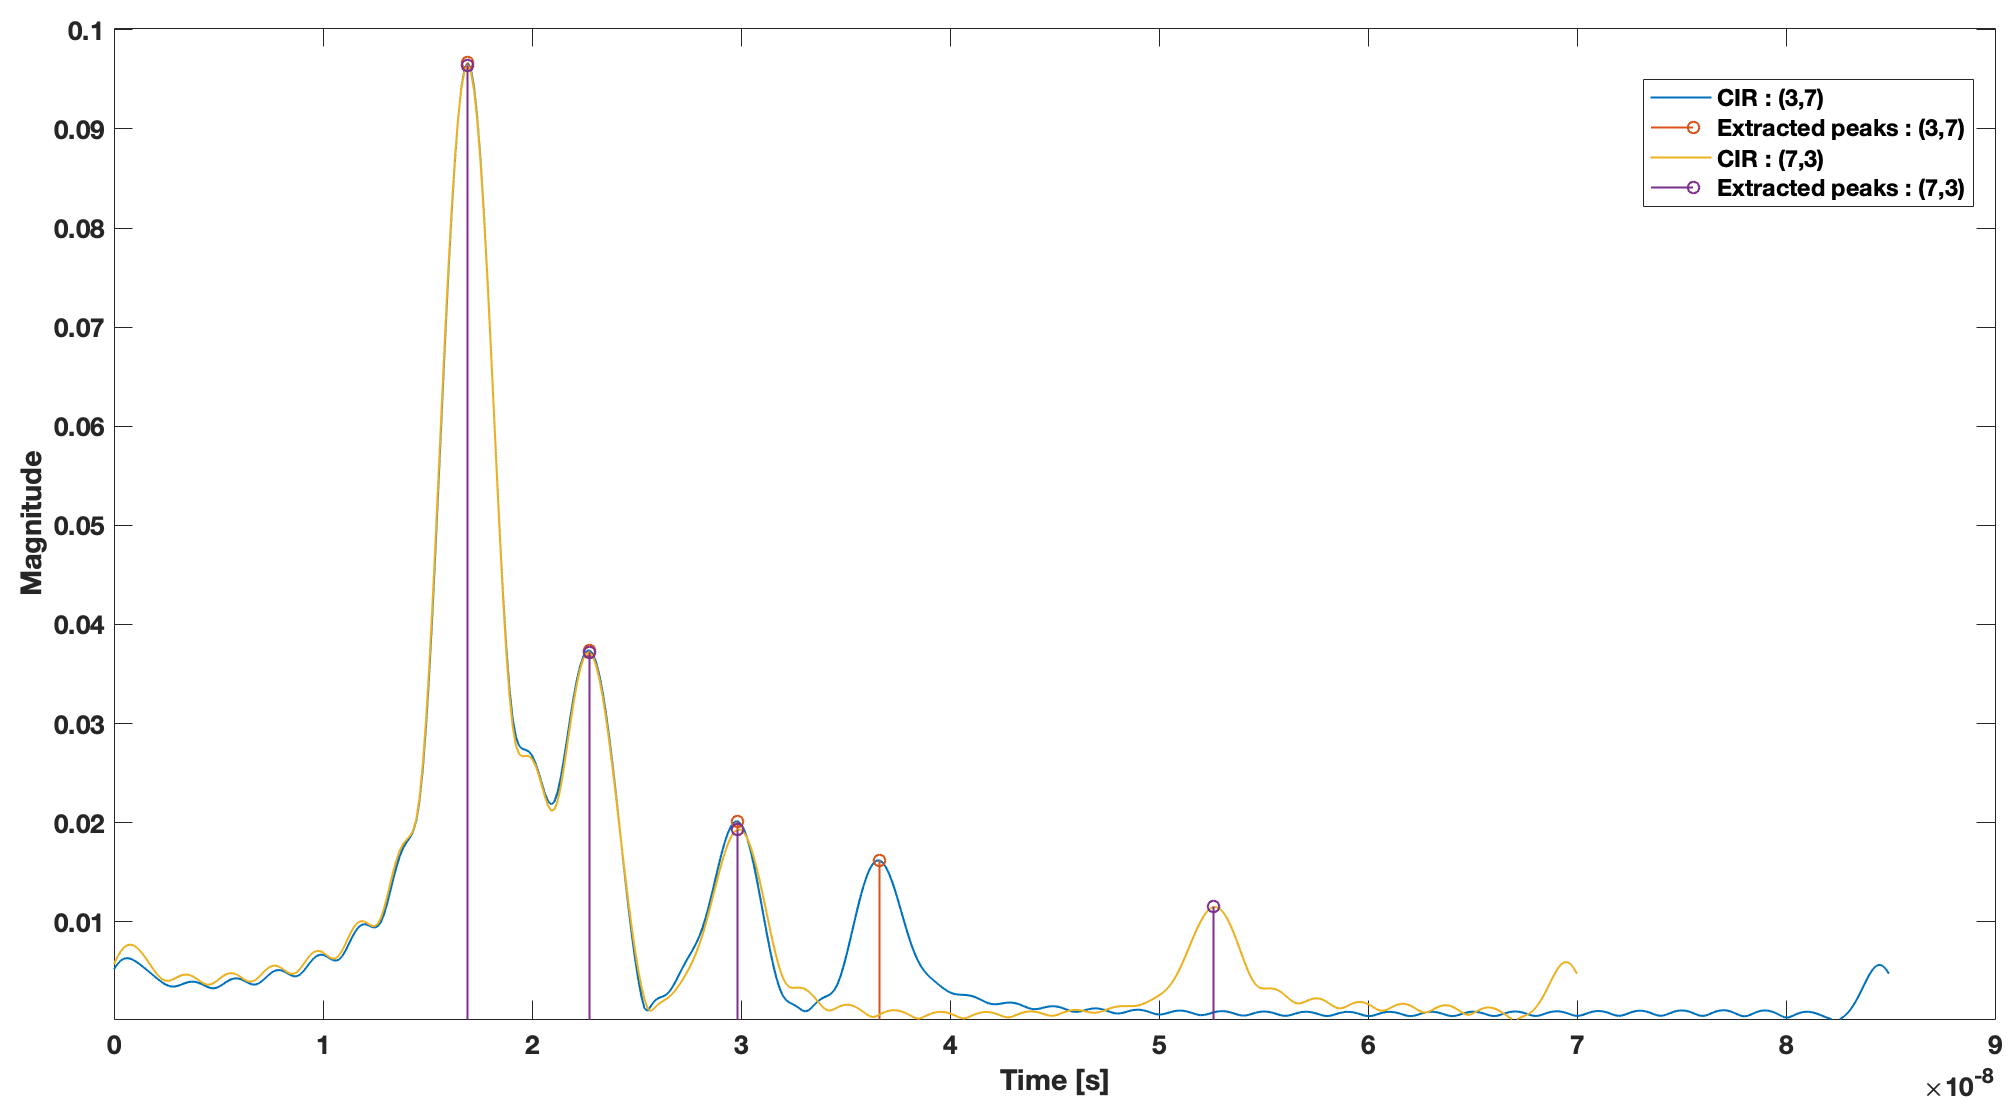
\includegraphics[width=.9\linewidth]{Images/cir_comparison_rect.png}
\caption{Comparison between two CIR obtained in a rectangular room (10 by 15)m. The anchor being located in (2, 2). \label{fig:rect_sym}}
\end{figure}

\subsection{Soft localization in an empty room}
\label{soft_empty_room}
Fig. \ref{fig:pos_ant_empty_non_sym} represents a room of 10 by 15 m dimension, with an anchor which is not set on any axis of symmetry. The chosen location of the anchor, which is (3, 1), is arbitrary and has mostly been chosen to avoid any location suffering from the symmetry. As we can observe, more than half of the location were correctly found back and more than two third were almost correctly found back\footnote{Exactly 86 over 150 were correctly found back and 115 over 150 was almost correctly found back. Almost meaning that the max distance between the tag and its location estimation is at most 1.5m.}.

\begin{figure}[H]
\centering
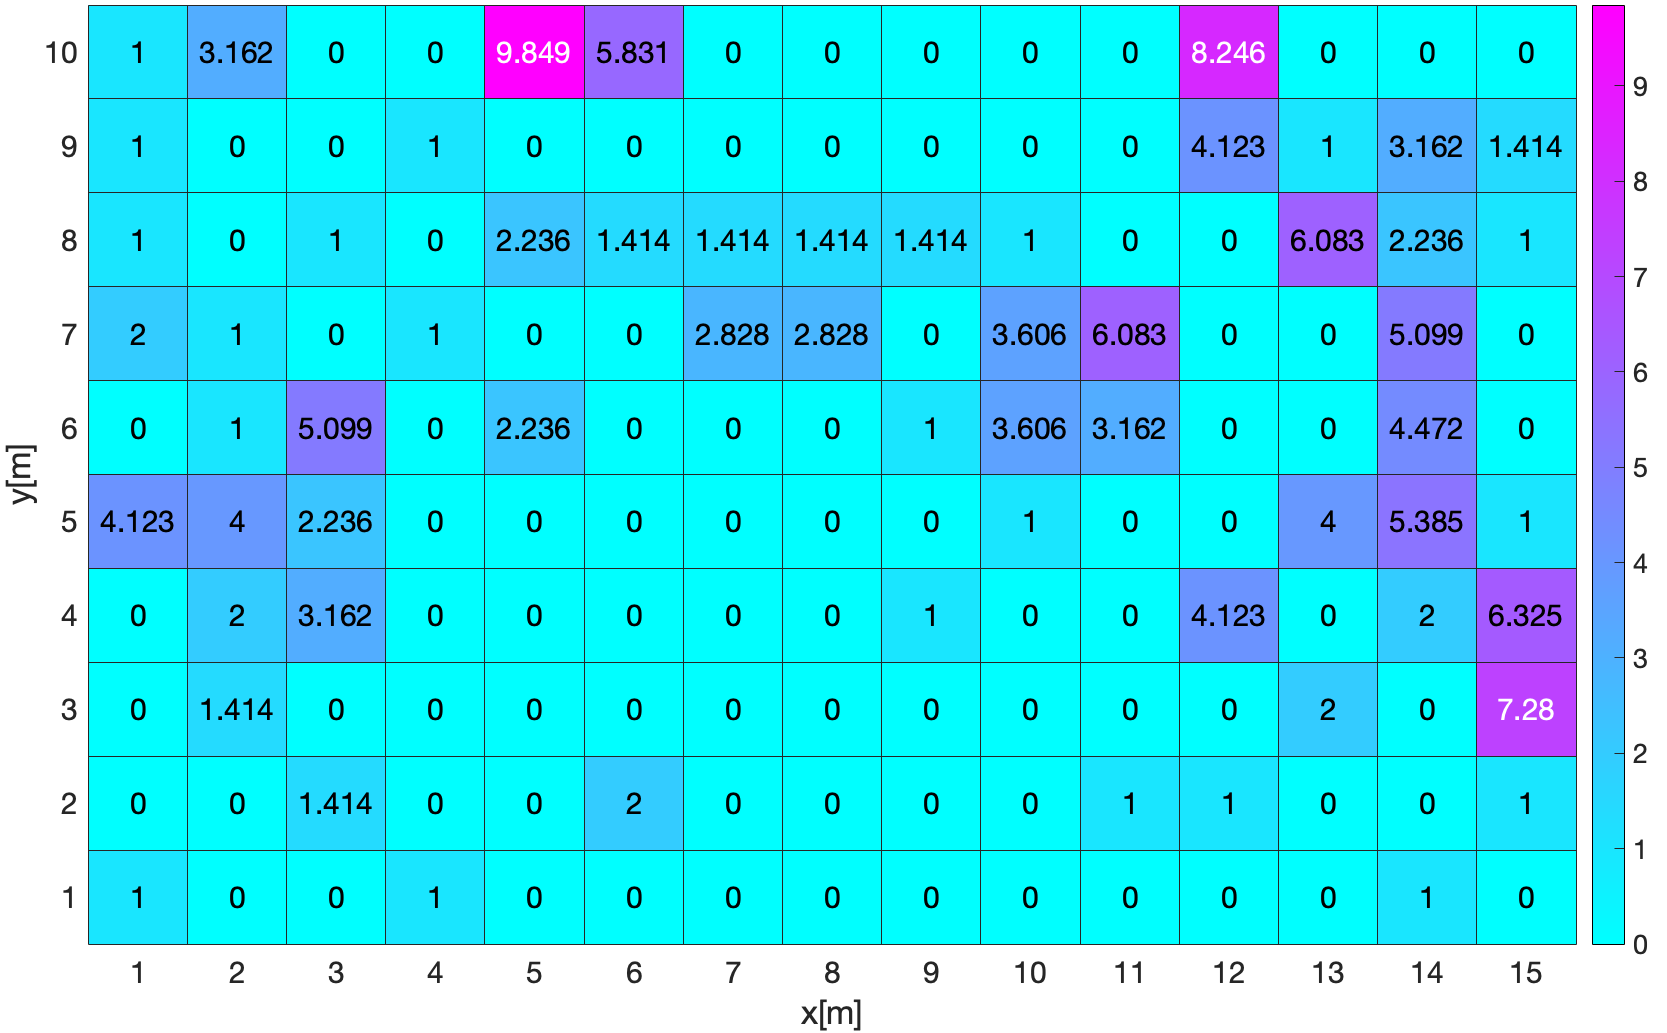
\includegraphics[width=\linewidth]{Images/no_more_name_idea.png}
\caption{Distance [m] between the tag location and its estimation using the \gls{sla}. Anchor being located in (3, 1). \label{fig:pos_ant_empty_non_sym}}
\end{figure}

We can observe that some locations have a relatively big error in comparison with the size of the room. For example, at the point (15, 3), the error made is about 7.3 m. To analyse the source of the error, a map of the \gls{mse} computed between the realistic \gls{cir} and the theoretical \gls{cir} computed at each location is drawn on Fig. \ref{fig:mse_analysis}. We can see that the best \gls{mse} is located at (13, 10) instead of the (15, 3) expected which corresponds to the distance error of 7.3 m.

\begin{figure}[H]
\centering
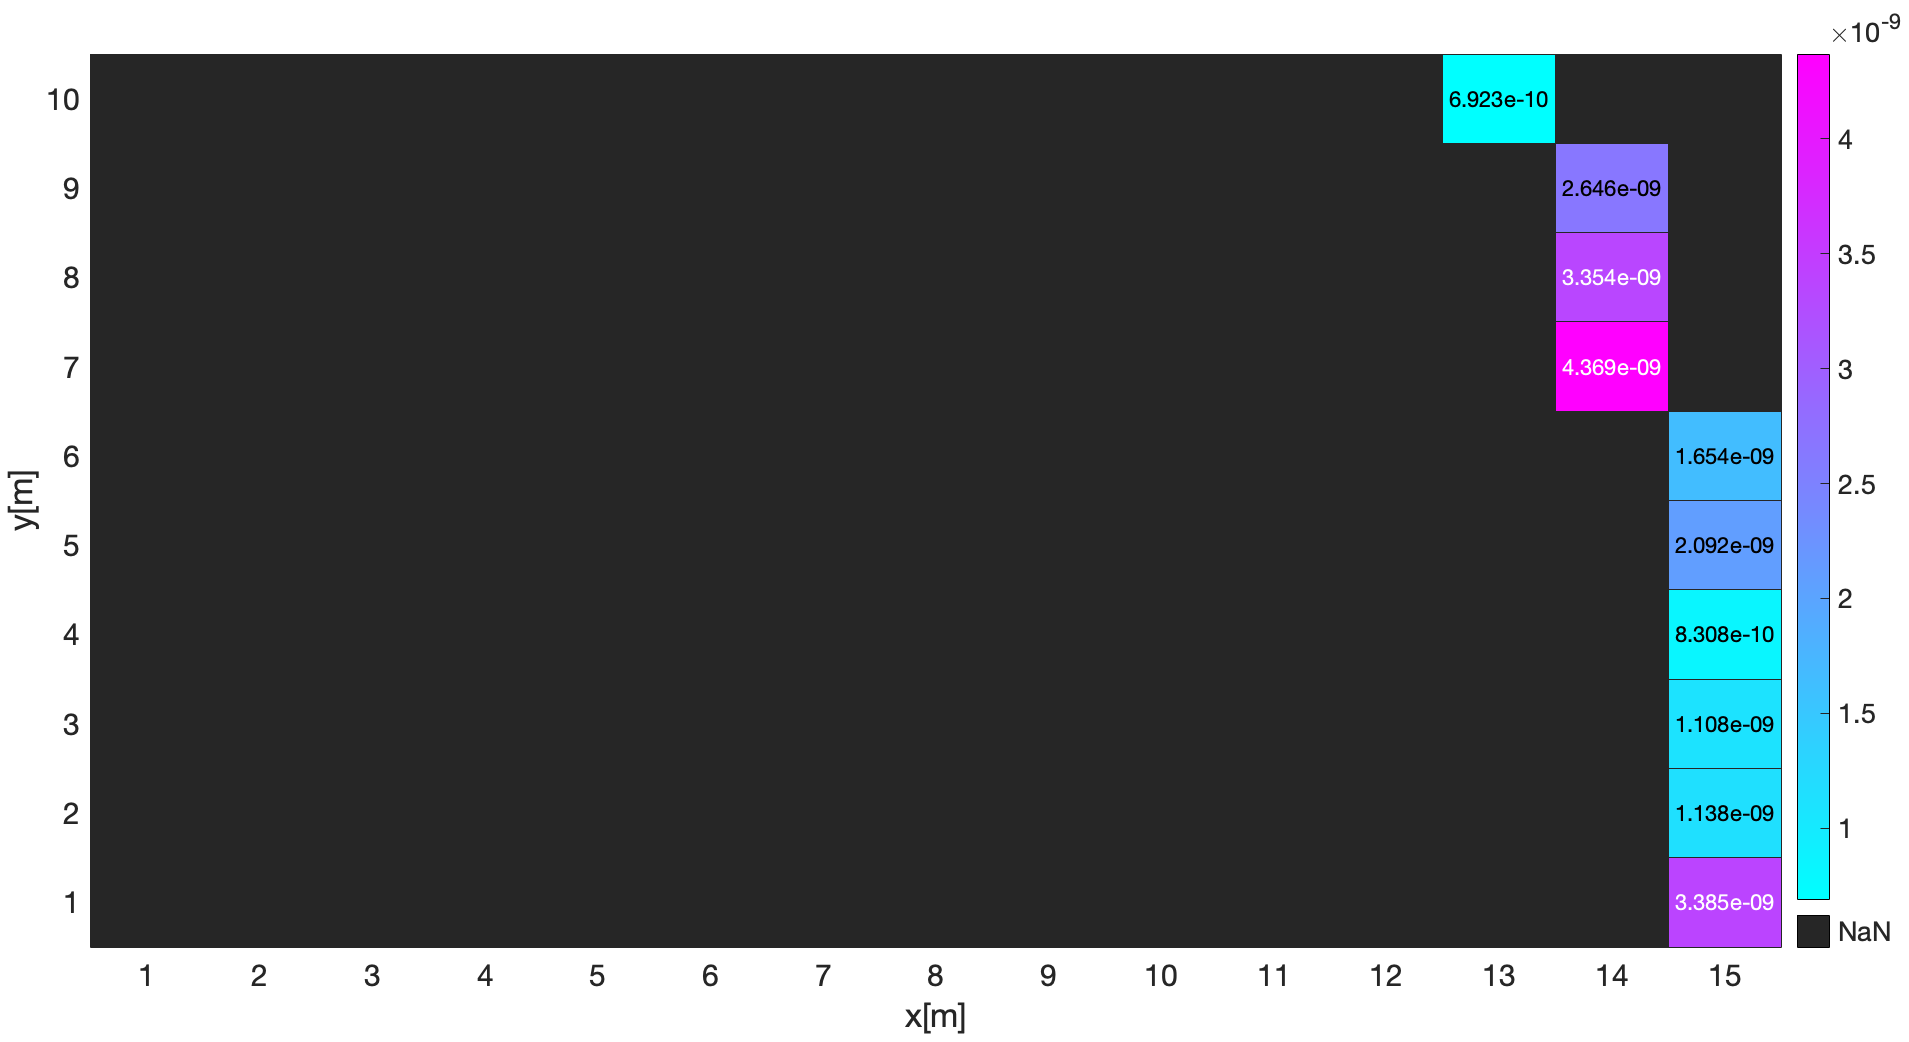
\includegraphics[width=\linewidth]{Images/no_name_1.png}
\caption{MSE map generated with an anchor in (2, 2) and the tag being located at (8, 4). The room configuration is an empty rectangle of 15 by 10 m. \label{fig:mse_analysis}}
\end{figure}

It can be interesting to compare the full \gls{cir} instead of only comparing the peaks. This is what is shown on Fig. \ref{fig:cir_compa}, the top \gls{cir} being the realistic, the middle corresponding to the \gls{cir} originating from the tag exact location while the bottom \gls{cir} corresponds to the one at coordinates (13, 10), where the best \gls{mse} can be found.

\begin{figure}[H]
\centering
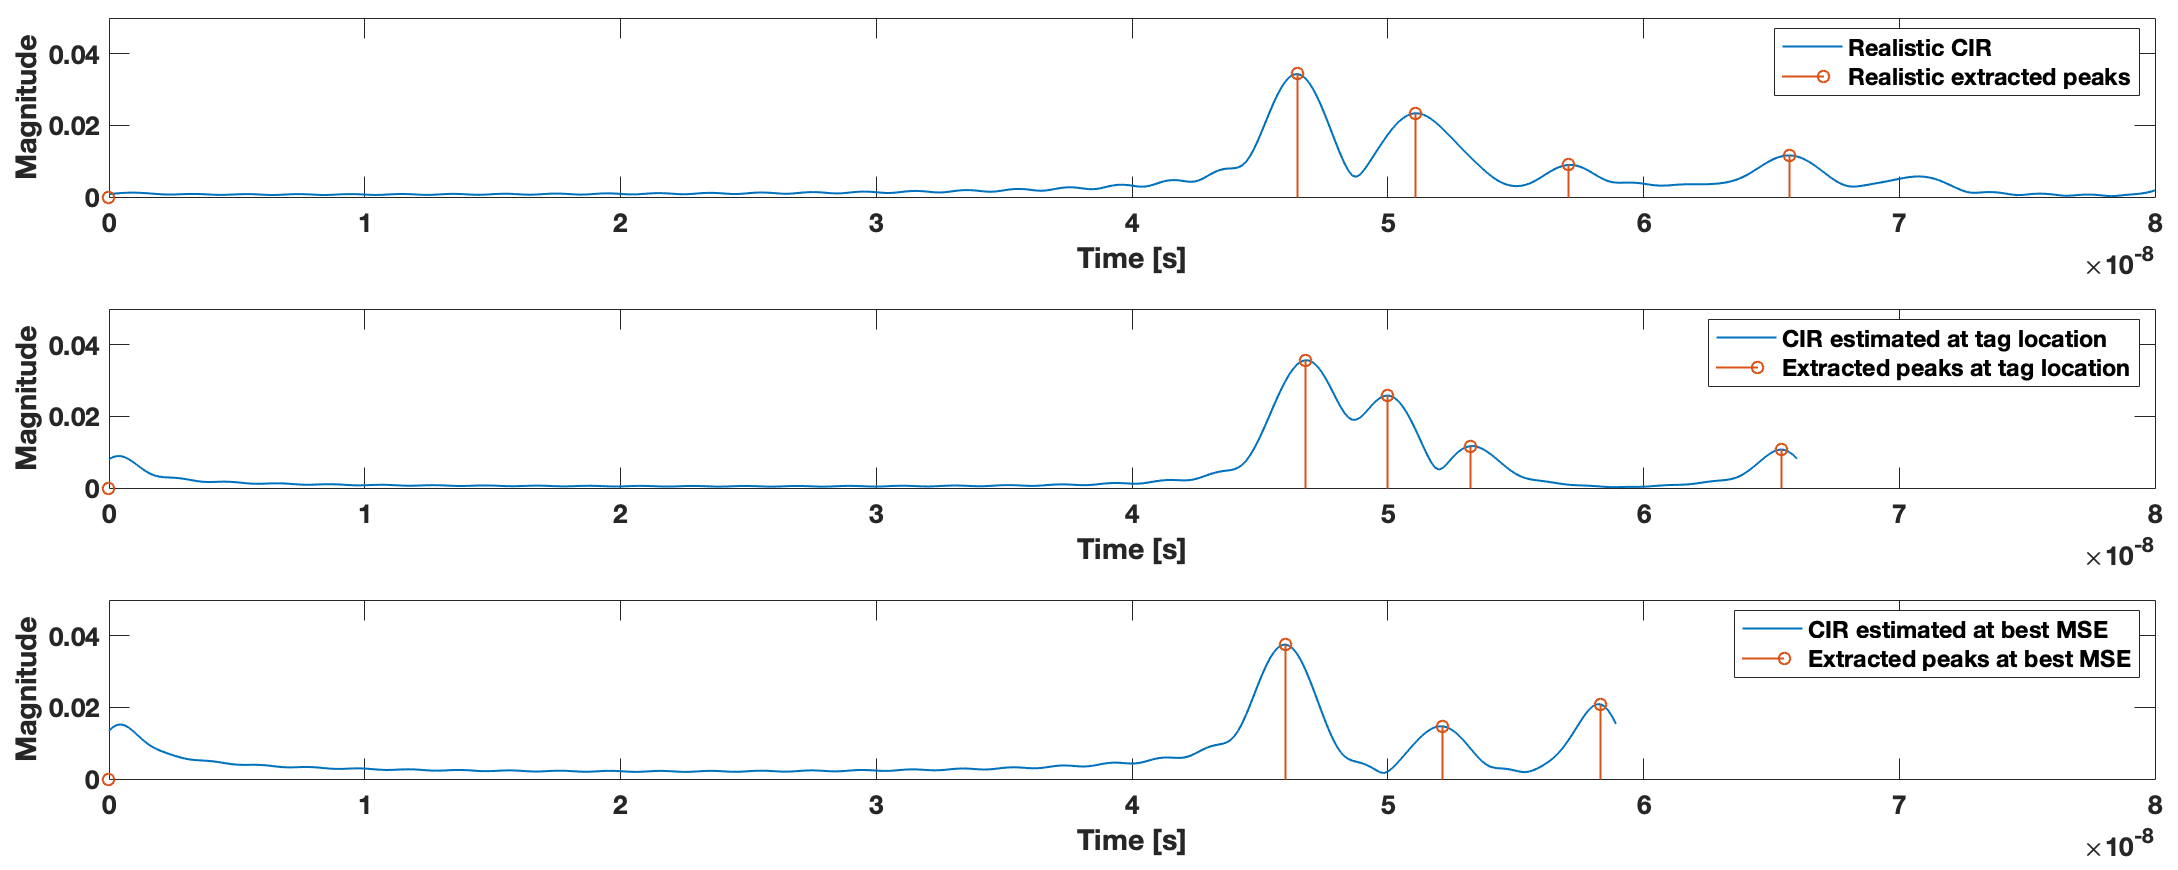
\includegraphics[width=\linewidth]{Images/no_name_2.png}
\caption{CIR comparison between the realistic CIR, the theoretical CIR at the best MSE (the estimated tag location) and the theoretical CIR at the real tag location. \label{fig:cir_compa}}
\end{figure}

Several observations can be made. First of all,, it can be seen that the form of the middle \gls{cir} does not fully correspond to the top \gls{cir}. Those difference in the form can mostly be attributed to the multiple reflections that take place in the top \gls{cir}. From that moment, if the two \gls{cir} are too different, the \gls{sla} will have some difficulties to compare them and find a theoretical \gls{cir} that really matches the realistic.
\vspace{2mm}

About the bottom \gls{cir}, this have been chosen by the algorithm as the best one by default. Since no \gls{cir} stood out, meaning that the extracting peaks from the theoretical \gls{cir} did not fully correspond to the realistic as in \ref{fig:soft_simu}, the less worst in term of \gls{mse} was chosen.
\vspace{2mm}

\subsubsection{Soft part of the algorithm}

This algorithm is call soft because of the \gls{mse} map produced as in Fig. \ref{fig:mse_analysis}. Instead of going back the location where the \gls{mse} has the lowest value, we could evaluate the area where the \gls{mse} is the average minimal.
\vspace{2mm}

In this example, while the location (13, 10) clearly has the lowest \gls{mse}, (15, 4) also has a \gls{mse} of magnitude $10^{-8}$. It also appears that (15, 4) is surrounded by some relatively low \gls{mse} values. We could therefore use this algorithm not only based on the lowest \gls{mse} computed but also based on the probability to be in a specific area filled with low \gls{mse} values.
\vspace{2mm}

This solution is not optimal and may not solve every possible location. For example, Fig. \ref{fig:again_an_image} shows the \gls{mse} map for the tag location (14, 6). The estimated location being (15, 2) would not slightly differ using this probability map.

\begin{figure}[H]
\centering
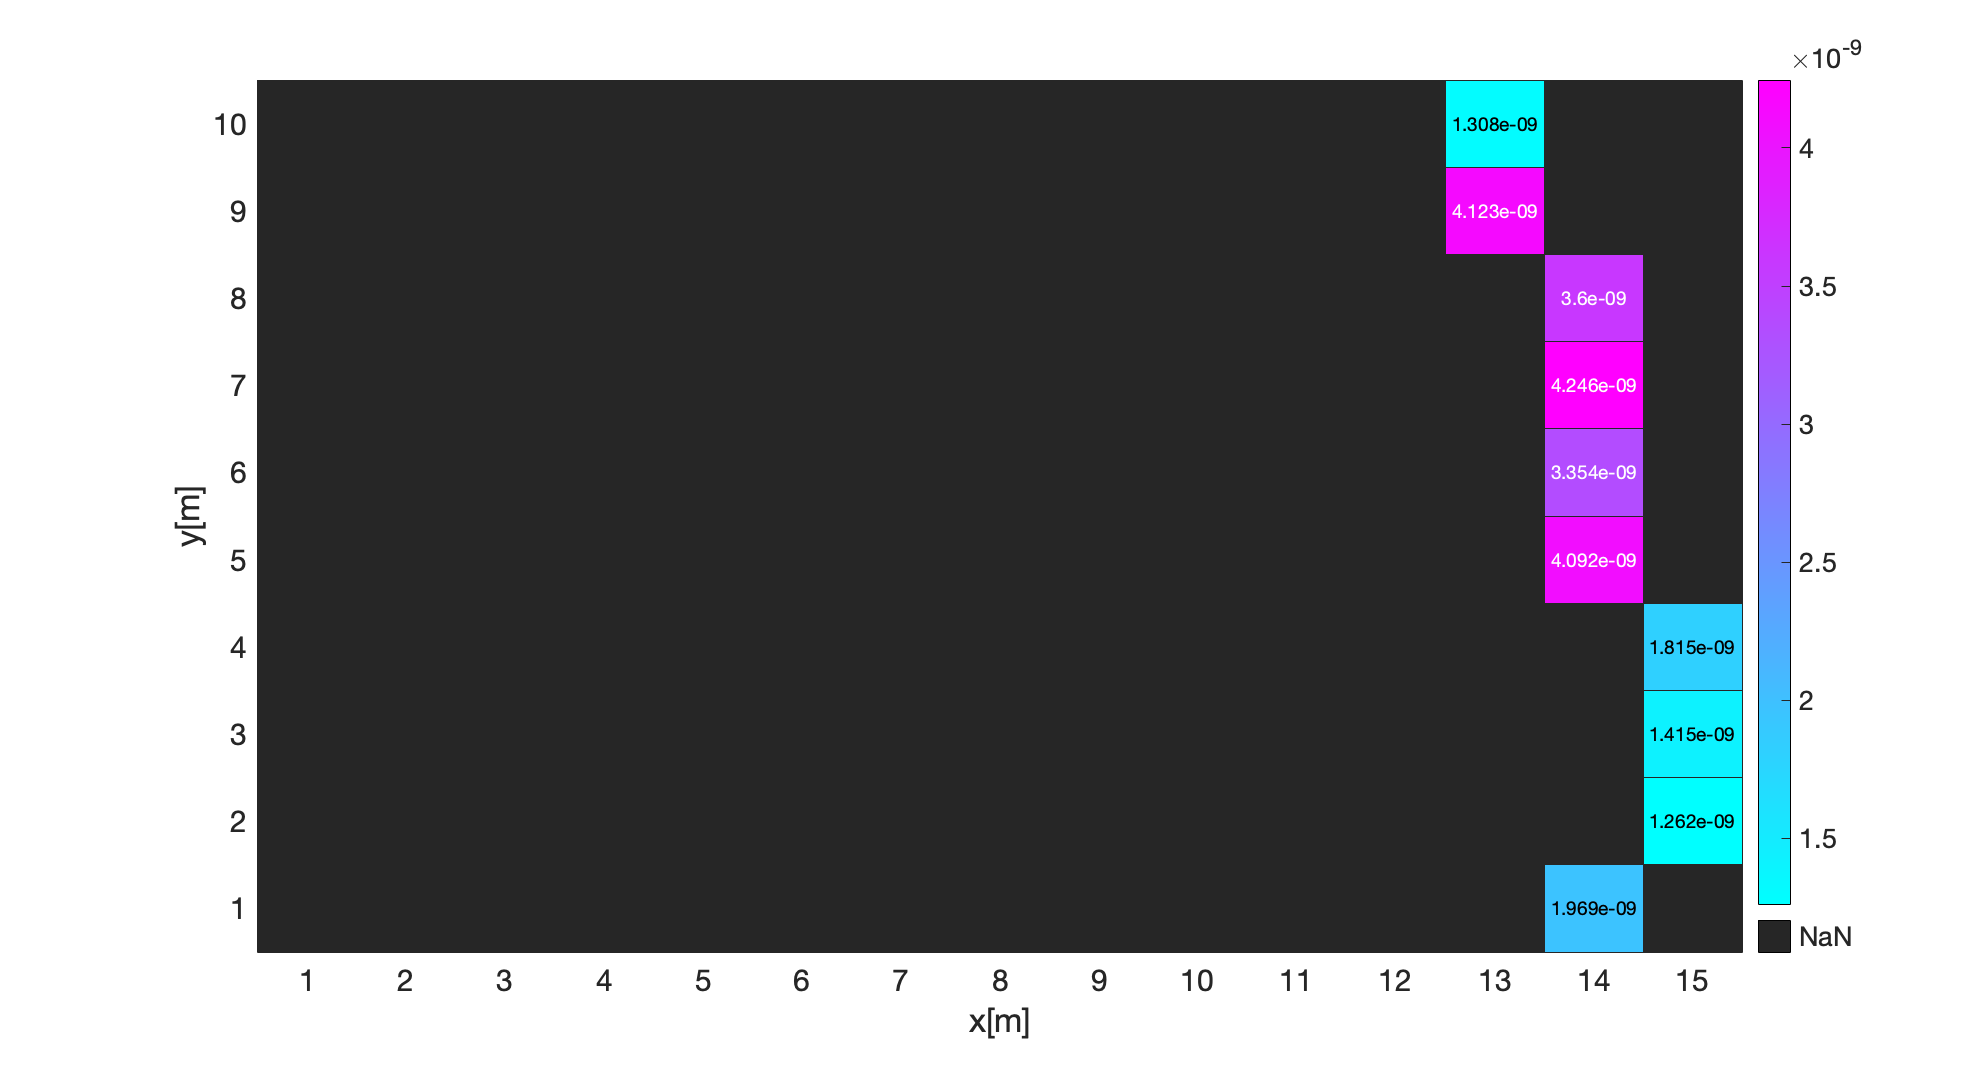
\includegraphics[width=.9\linewidth]{Images/image_XXX.png}
\caption{MSE map generated with an anchor in (2, 2) and the tag being located at (14, 6). The room configuration is an empty rectangle of 15 by 10 m. \label{fig:again_an_image}}
\end{figure}

Eventually, in a perfect non cluttered room, the \gls{sla} does not reach a perfect score on the localization in comparison with the three anchor model in \cite{hannotier2019indoor}. It may be possible to improve the localisation and give a trustful interval based on a \gls{mse} map as in Fig. \ref{fig:cir_compa}.

\subsection{Soft localization in a cluttered room}
\label{simu_soft_clut}
The simulations of this section have been done for a room with the same dimension as section \ref{soft_empty_room} filled with furniture. Four different consoles of various sizes are placed against each wall of the room. This will results in are realistic \gls{cir} being more complex because of the various reflections happening on the walls and the furniture. The used room can be seen in Fig. \ref{fig:room_cluttered}.

\begin{figure}[H]
\centering
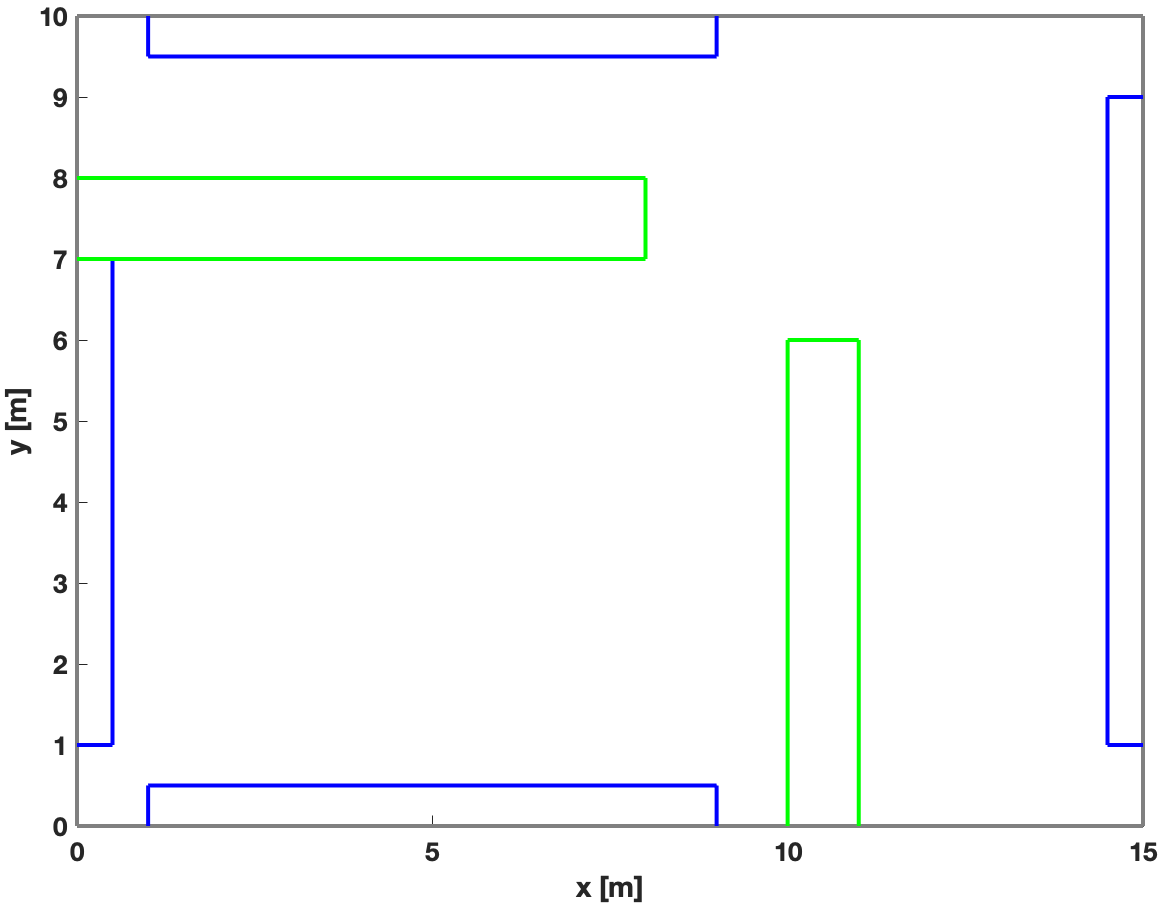
\includegraphics[width=.6\linewidth]{Images/room_furniture.png}
\caption{Furniture displayed in the room. \label{fig:room_cluttered}}
\end{figure}


The set anchor has been located at the same place as in the previous section and taken into account furniture that are in blue. As we can observe in Fig. \ref{fig:dist_clut_room}, the quality of the localization lowers, this quality decreases even more when furniture are set in the middle of the room, as it can be seen on Fig. \ref{fig:dist_lot_clut_room}, creating more and more surface where reflection can take place.

\begin{figure}[H]
\centering
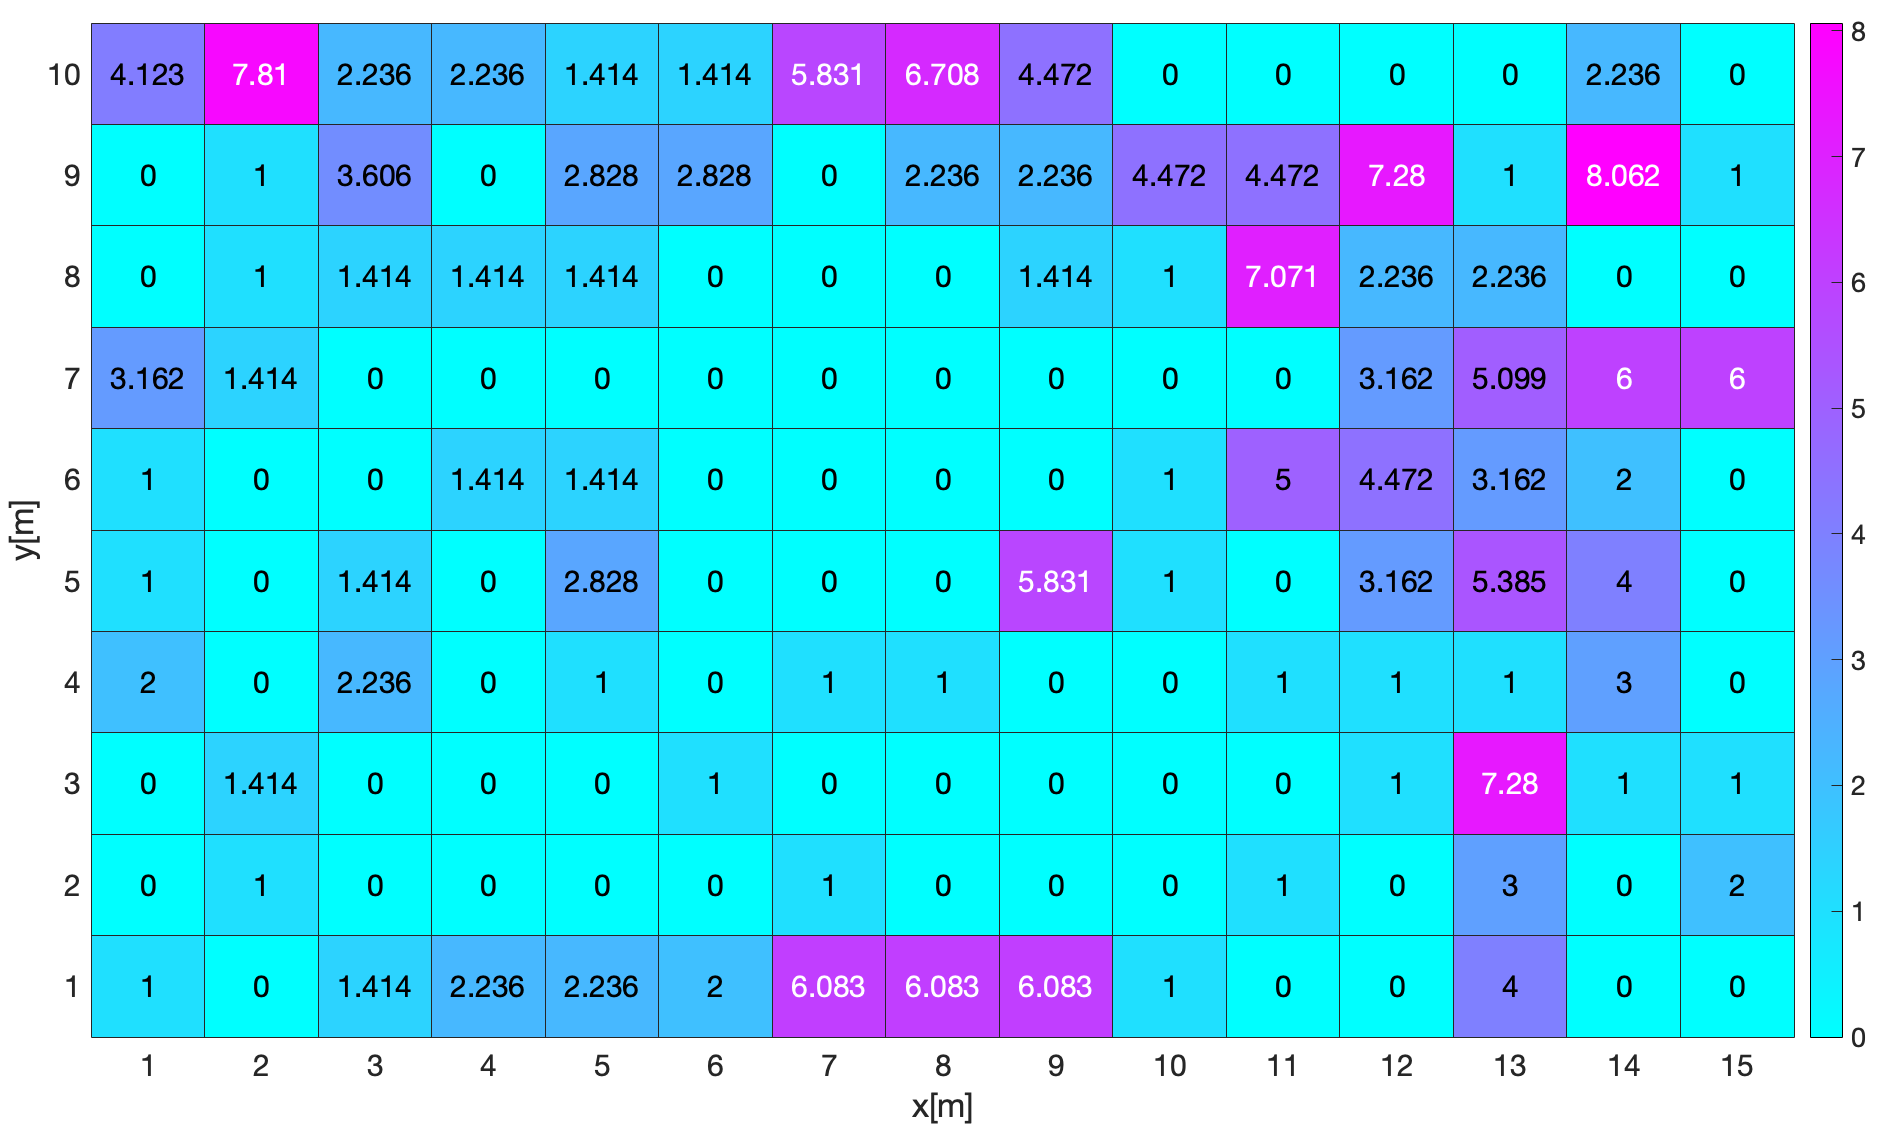
\includegraphics[width=.9\linewidth]{Images/cluttered_room.png}
\caption{Distance [m] between the real position of the tag and its estimation using the \gls{sla}. The room configuration has only the blue furniture from Fig. \ref{fig:room_cluttered}.
\label{fig:dist_clut_room}}
\end{figure}

\begin{figure}[H]
\centering
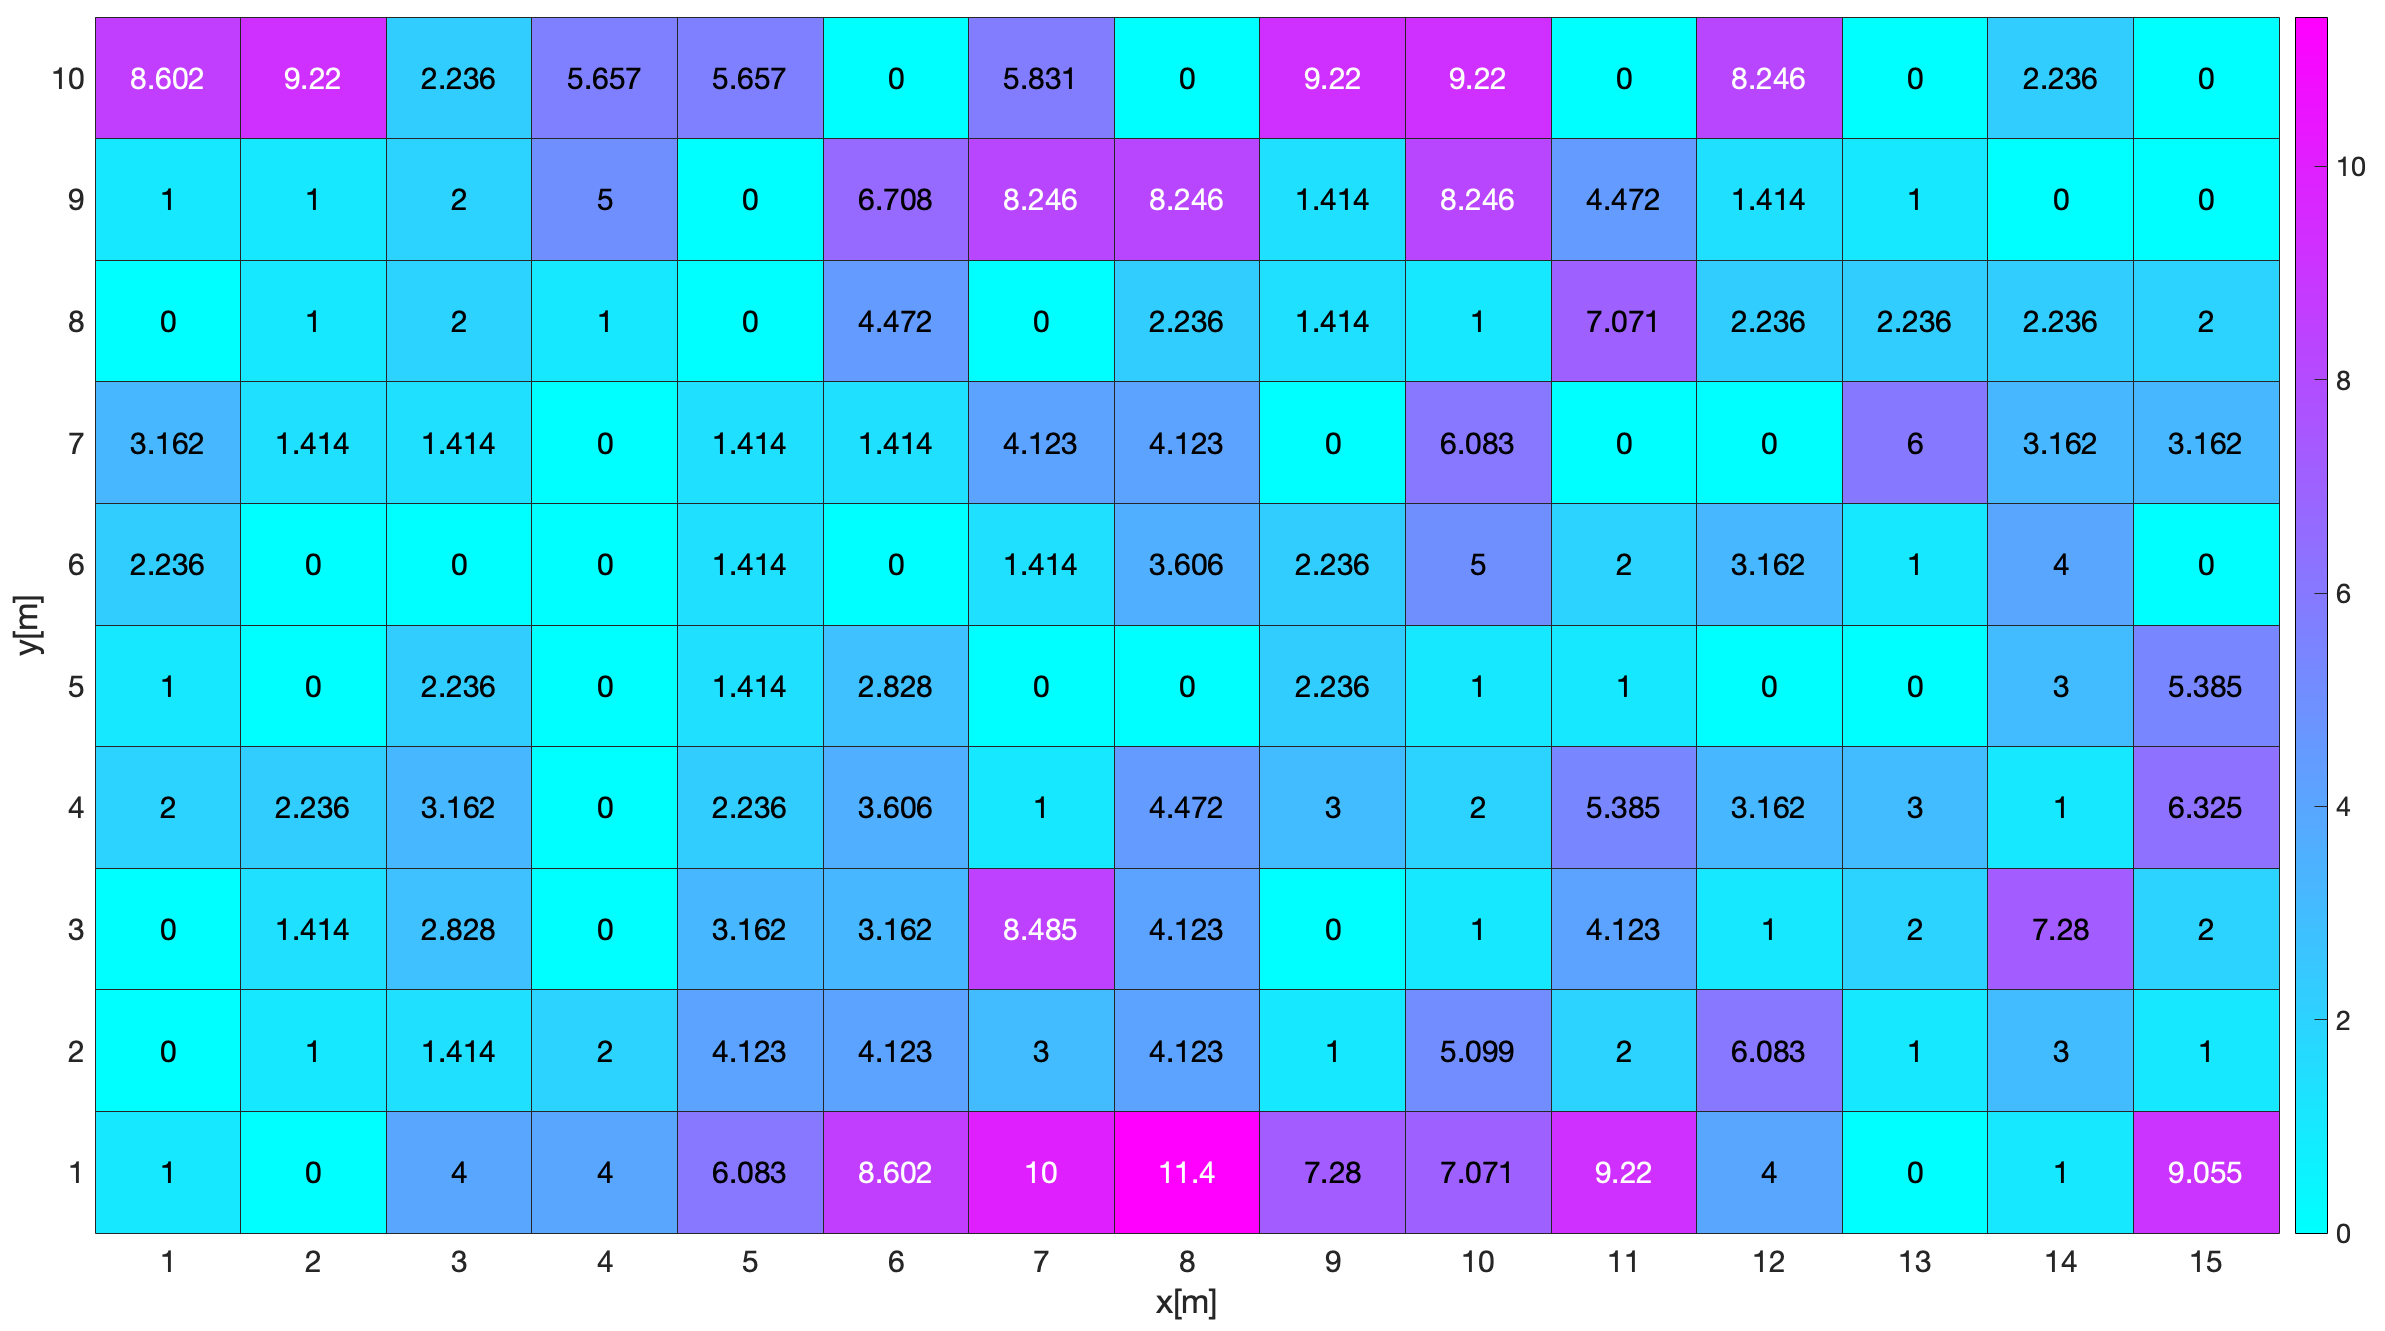
\includegraphics[width=.9\linewidth]{Images/sla_cluttered_lot.png}
\caption{Distance [m] between the real position of the tag and its estimation using the \gls{sla}. The room configuration has all the furniture from Fig. \ref{fig:room_cluttered}.\label{fig:dist_lot_clut_room}}
\end{figure}

This evolution can be understood by checking the realistic \gls{cir} obtained for different versions of the room for different locations of the tag. On Fig. \ref{fig:cir_comp_dif_room_working}, those \gls{cir} can be seen for the coordinates (10, 4), a more or less well estimated tag location.

\begin{figure}[H]
\centering
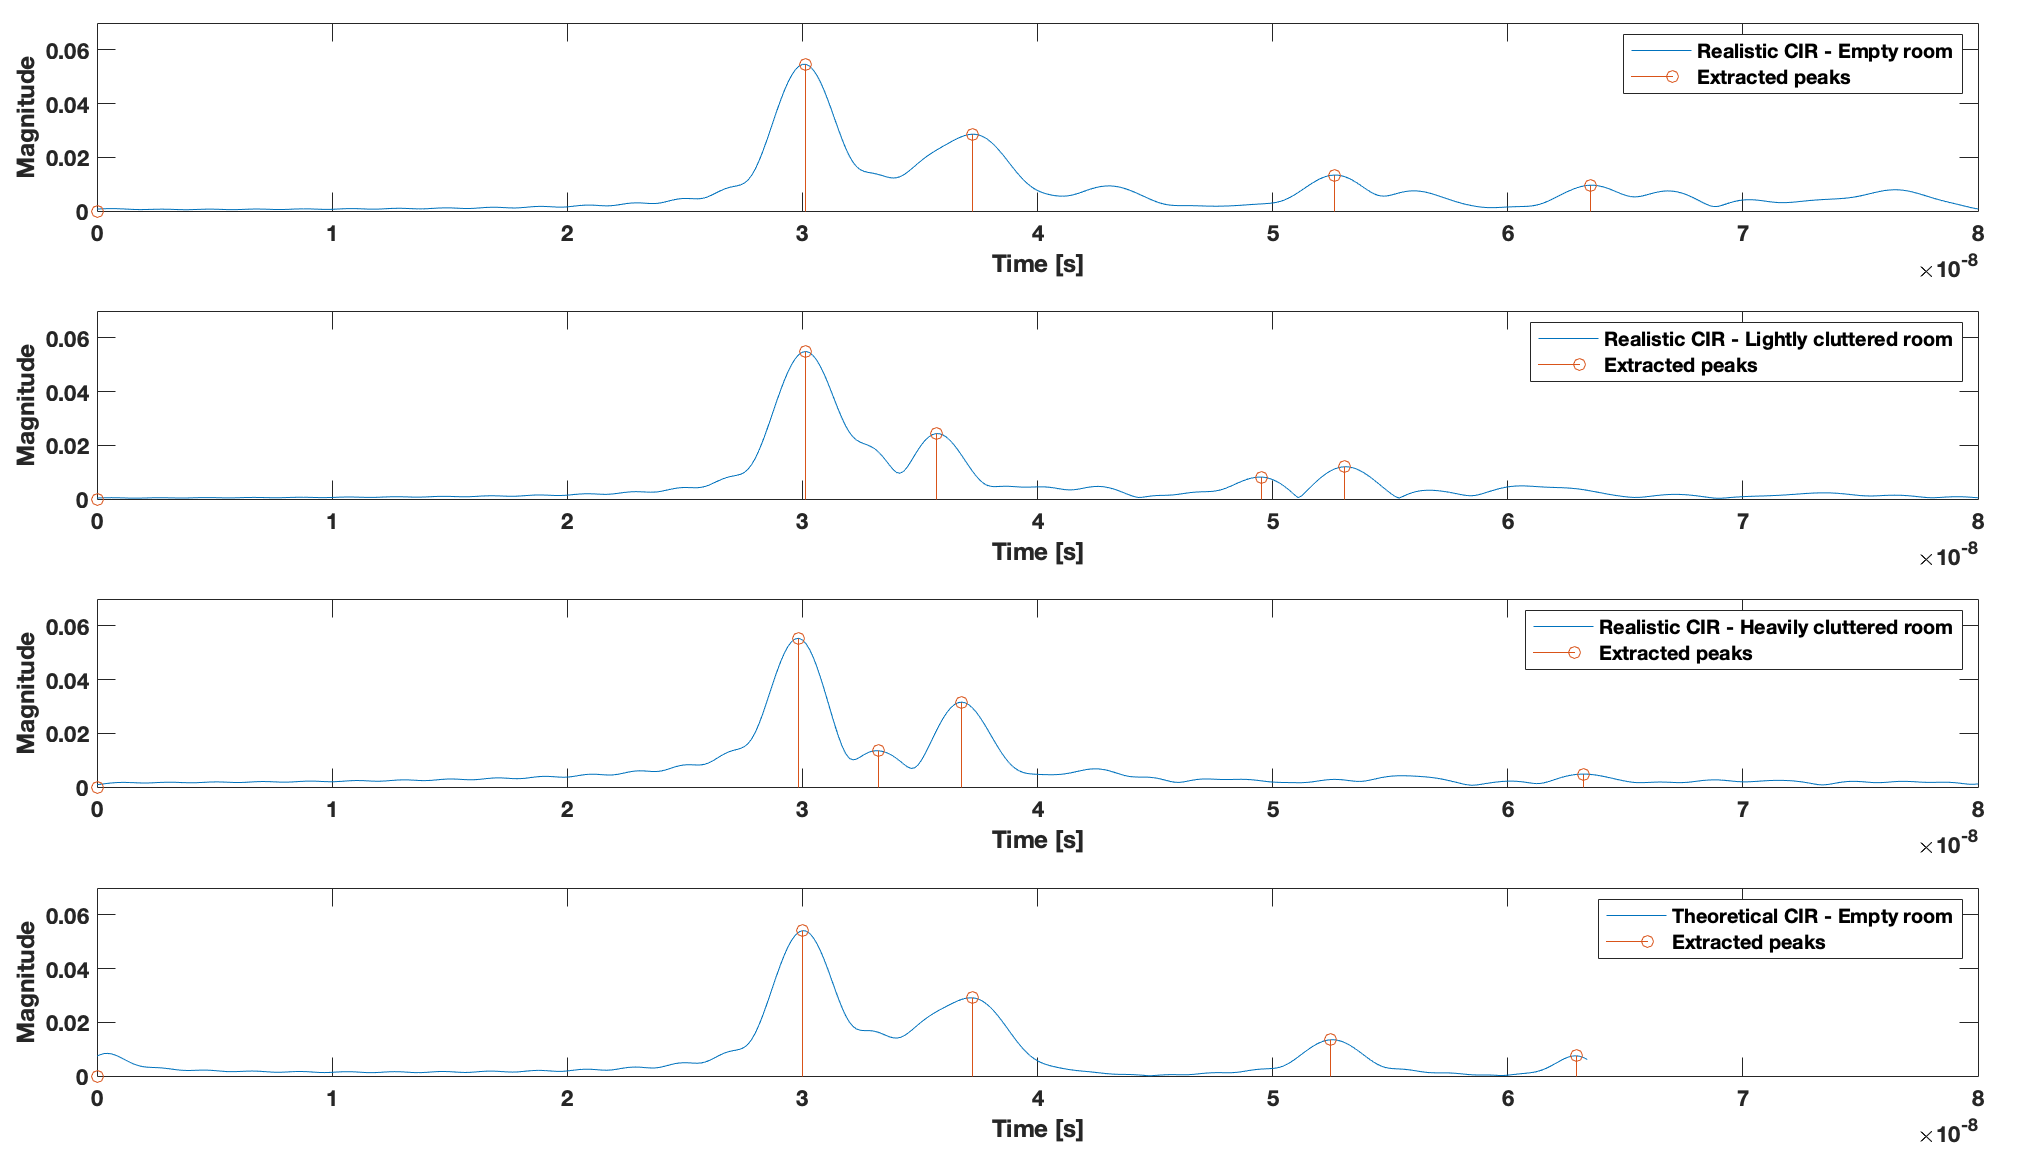
\includegraphics[width=.85\linewidth]{Images/cir_success_comparison.png}
\caption{CIRs obtained for an anchor set at (1, 3) and a tag at (10, 4). The top three are the realistic CIR obtained, from top to bottom respectively in an empty room, a room with blue furniture from Fig. \ref{fig:room_cluttered} and a room with all the furniture set. Fourth CIR is the theoretical CIR obtained using an empty room.  \label{fig:cir_comp_dif_room_working}}
\end{figure}

As we can observe, the \gls{cir} change a lot according to the cluttering of the room. The more cluttering there is, the more it changes. This explains the loss in precision as the room is more and more filled with extra furniture. By looking at the second and third \gls{cir} of \ref{fig:cir_comp_dif_room_working}, we can see that while the first more or less matches the fourth \gls{cir}, the general form keeps changing. The peaks are moved, are mingled, attenuated because of the transmission trough the furniture lowers some peaks and new peaks are created. All those effects significantly change the form of the \gls{cir}.

\begin{figure}[H]
\centering
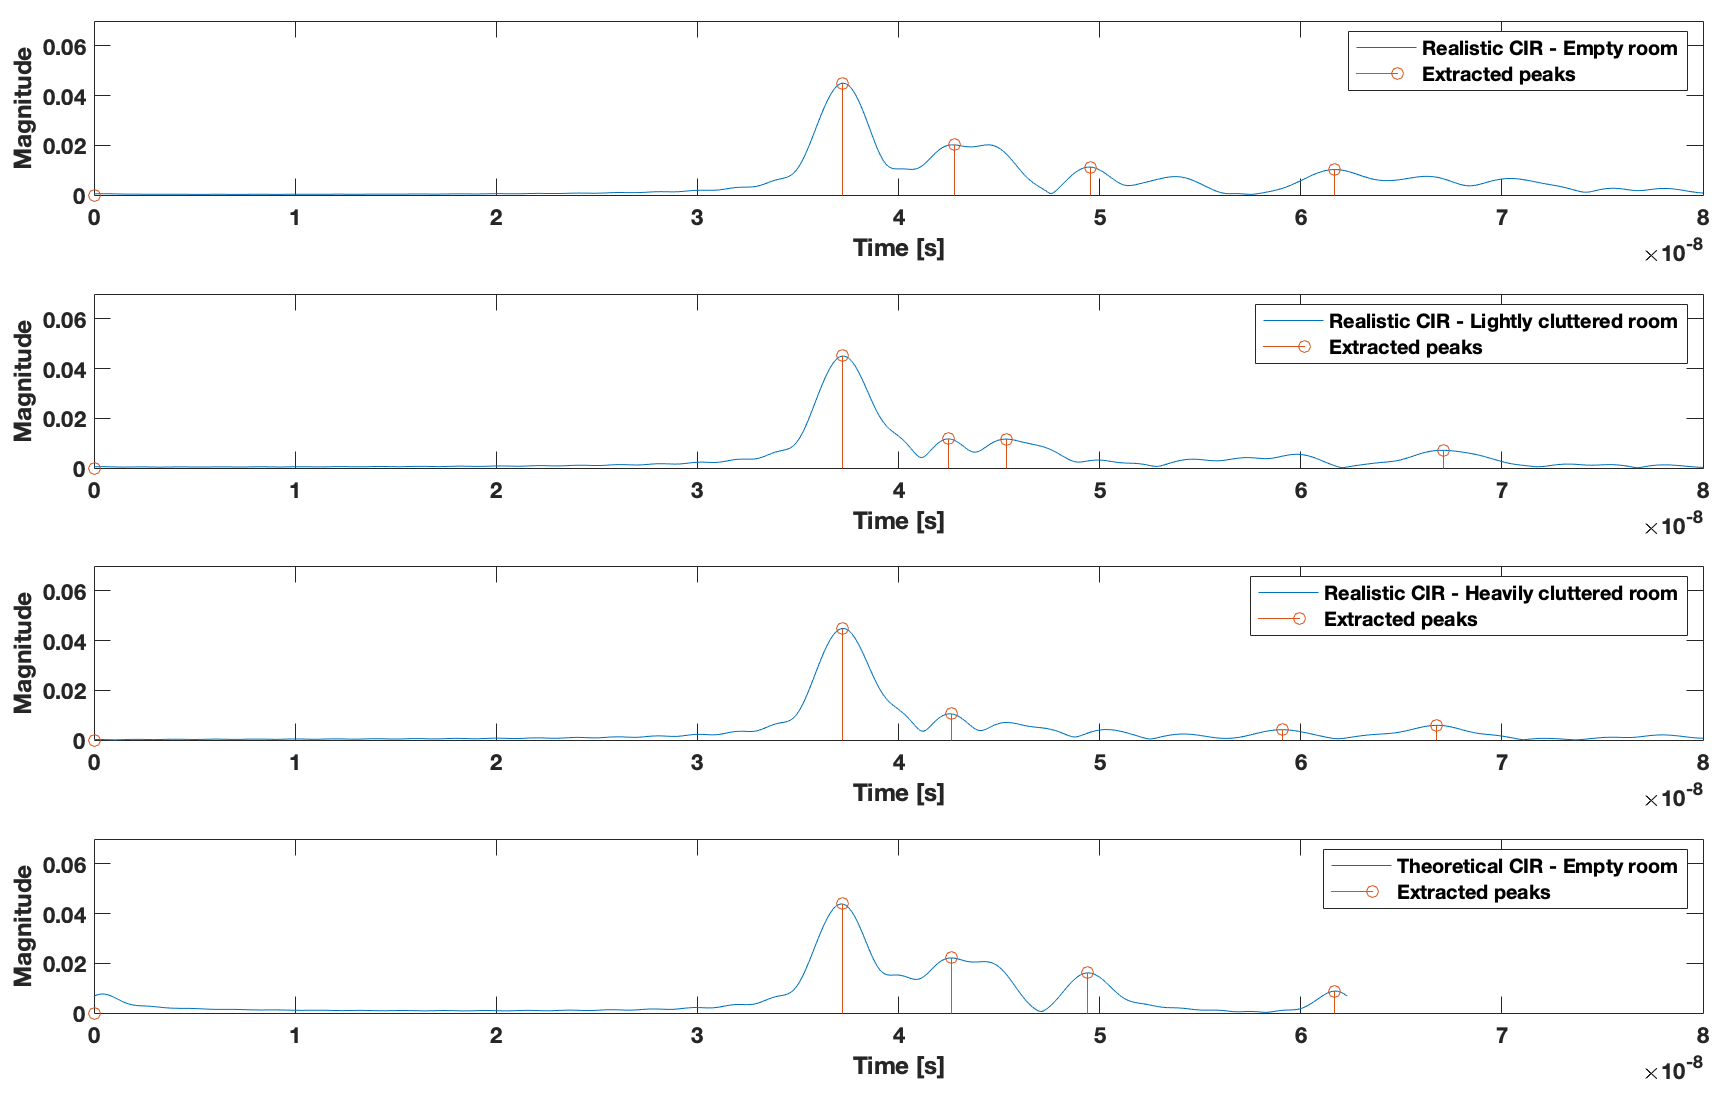
\includegraphics[width=.85\linewidth]{Images/cir_failed_comparison.png}
\caption{CIRs obtained for an anchor set at (1, 3) and a tag at (11, 8). The top three are the realistic CIR obtained, from top to bottom respectively, in an empty room, a room with blue furniture from Fig. \ref{fig:room_cluttered}  and a room with all the furniture set. Fourth CIR is the theoretical CIR obtained using an empty room. \label{fig:cir_comp_dif_room_failing}}
\end{figure}

When comparing the localization performance for a tag placed in (10, 4) and a tag placed in (11, 8), it quickly appears that the difference originates in the shape of the \gls{cir}. This shape may vary a lot according to the setting of the tag,  the walls, the furniture and obviously the anchor. 
\vspace{2mm}

Since the only parameter that can be influenced is the location of the anchor, this parameter has been changed and various simulations with different locations of the anchor has been generated. Those simulations can be seen in appendix \ref{app:sla}.
\vspace{2mm}

One the whole, the localization showed some better performances when there are not any walls in the middle of the room. In such room, the localization using one anchor appears to be really complicated and hazardous. This room configuration globally does not give any good results independently of the tag's location. A possible explanation is discussed in section \ref{simu_anal}.
\vspace{2mm}

From those simulations, we can compare several placements of the anchor. The first thing that can be concluded is that setting the anchor in the middle of the room is not an optimal choice, the wrong estimation of the location of the tag being more frequent than for the other possible locations of the anchor. About the choice between setting the anchor in a corner or near a wall, the optimal position is less obvious. Both possibilities happens to give some rather good and less good performances according to the location of the anchor, as it can be seen in Fig. C.3, C.4. The anchors being located at one meter from each other.
\vspace{2mm}

Generally speaking, the performances really vary from one situation to another, according  to the furniture of the room and the location of the anchor. This system has some room for improvement, the comparison between the \gls{cir} can be modified, the method to extract the peaks can also be changed or improved. The number of peaks extracted can also be a variable to investigate.


\section{Hard Simulation}

This section discuss the \gls{hla} developed in chapter \ref{algos}. As for the \gls{sla}, several places to set the anchors will be discussed in several room configurations, filled with furniture or empty. To provide some meaning comparisons, the room configurations are the same as in section \ref{soft_sim}.

\subsection{Symmetry issues}

As we can observe on Fig. \ref{fig:sym_hard} the same phenomenon occurs for the \gls{hla} and the \gls{sla}. A kind of symmetry appears across the bottom-left to top-right diagonal. On the lower side of this diagonal, the location outperformed in general the upper side. Which means that the symmetry will also be causing some troubles in this algorithm.
\vspace{2mm}

Since the generation of the different \gls{cir} is based on the same simulation for the \gls{sla} and the \gls{hla}, it is irrelevant to present the \gls{cir} of couple of mirror point around the axis of symmetry, this being already discussed in section \ref{sym_cases}. However, a significant difference between the Fig. \ref{fig:square_sym} and Fig. \ref{fig:sym_hard} resides in the black zone appearing in the results of the \gls{hla}.
\vspace{2mm}

As explained in section \ref{algo:hard}, this algorithm may not return any solution. We can observe that such locations are disposed symmetrically around the axis of symmetry. The origin of those unresolved solution are first studied by investigating the \gls{cir} of such places. 

\begin{figure}[H]
\centering
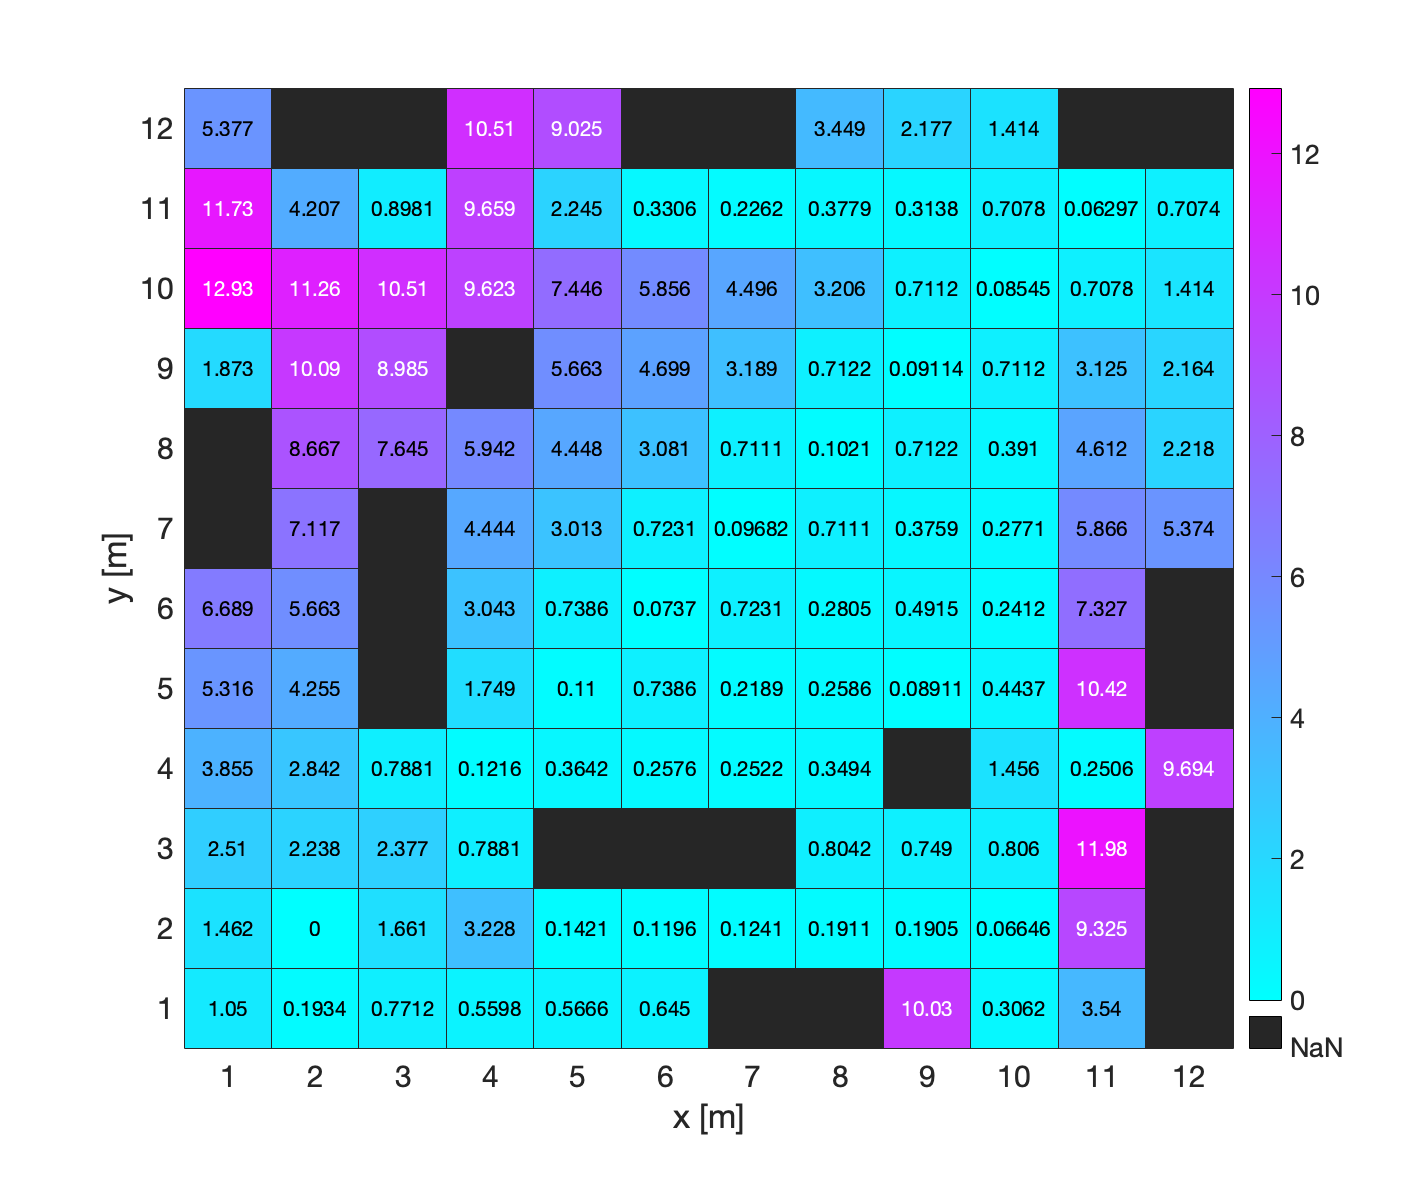
\includegraphics[width=.8\linewidth]{Images/hla_images/hla_anchor_(2_2)_empty.png}
\caption{Distance [m] between the tag exact location and the estimation provided by the \gls{hla}. Empty room of 12 by 12 meters, anchor set at (2, 2). Three peaks extracted. \label{fig:sym_hard}}
\end{figure}

On Fig. \ref{fig:cir_4_9}, the tag location (4, 9) is investigated. By observing the extracted peaks on the bottom figure, we can see that while the first and the third corresponds to some peaks in the theoretical \gls{cir}, the second is not match with any of them. This is the source of the error. 

\begin{figure}[H]
\centering
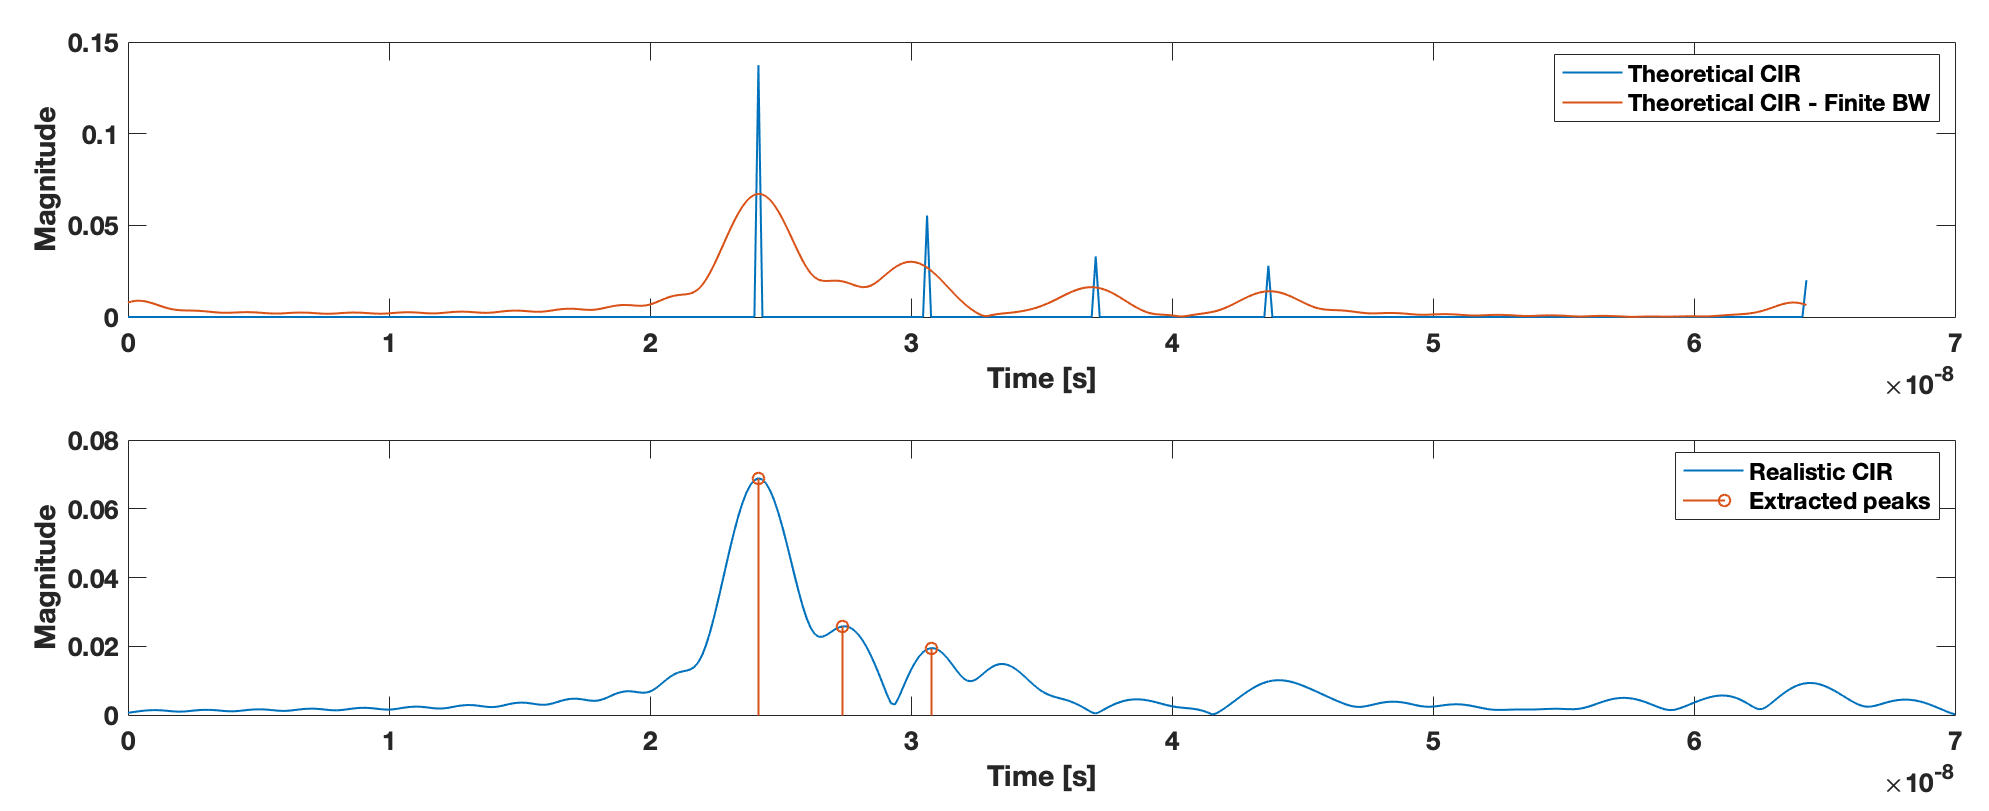
\includegraphics[width=.9\linewidth]{Images/hla_images/cir_4_9.png}
\caption{(Top) Theoretical CIR for an anchor set in (2, 2) and a tag set in (4, 9) in an empty room. Only the direct ray and signle reflections are generated. (Bottom) Realistic CIR generated in the same conditions. Up to three reflections taken, the extracted peaks are shown in orange.\label{fig:cir_4_9}}
\end{figure}

A possible solution, to avoid this outcome, which is not investigated here, would be to extract several other peaks from the realistic \gls{cir} in order to obtain a new system to solve. 

\subsection{Hard localization in an empty room}

In this section, the same configuration as the one used in the soft simulation is used. Several location for the anchor are compared, basically one in a corner (while avoiding the symmetry issue), another in the middle of wall and a last one being in the middle of the room. As we could expect, the anchor that sits in a corner has a better performance than the others. The middle of the room is prone to the symmetry as the middle of the different walls.

\begin{figure}[H]
\centering
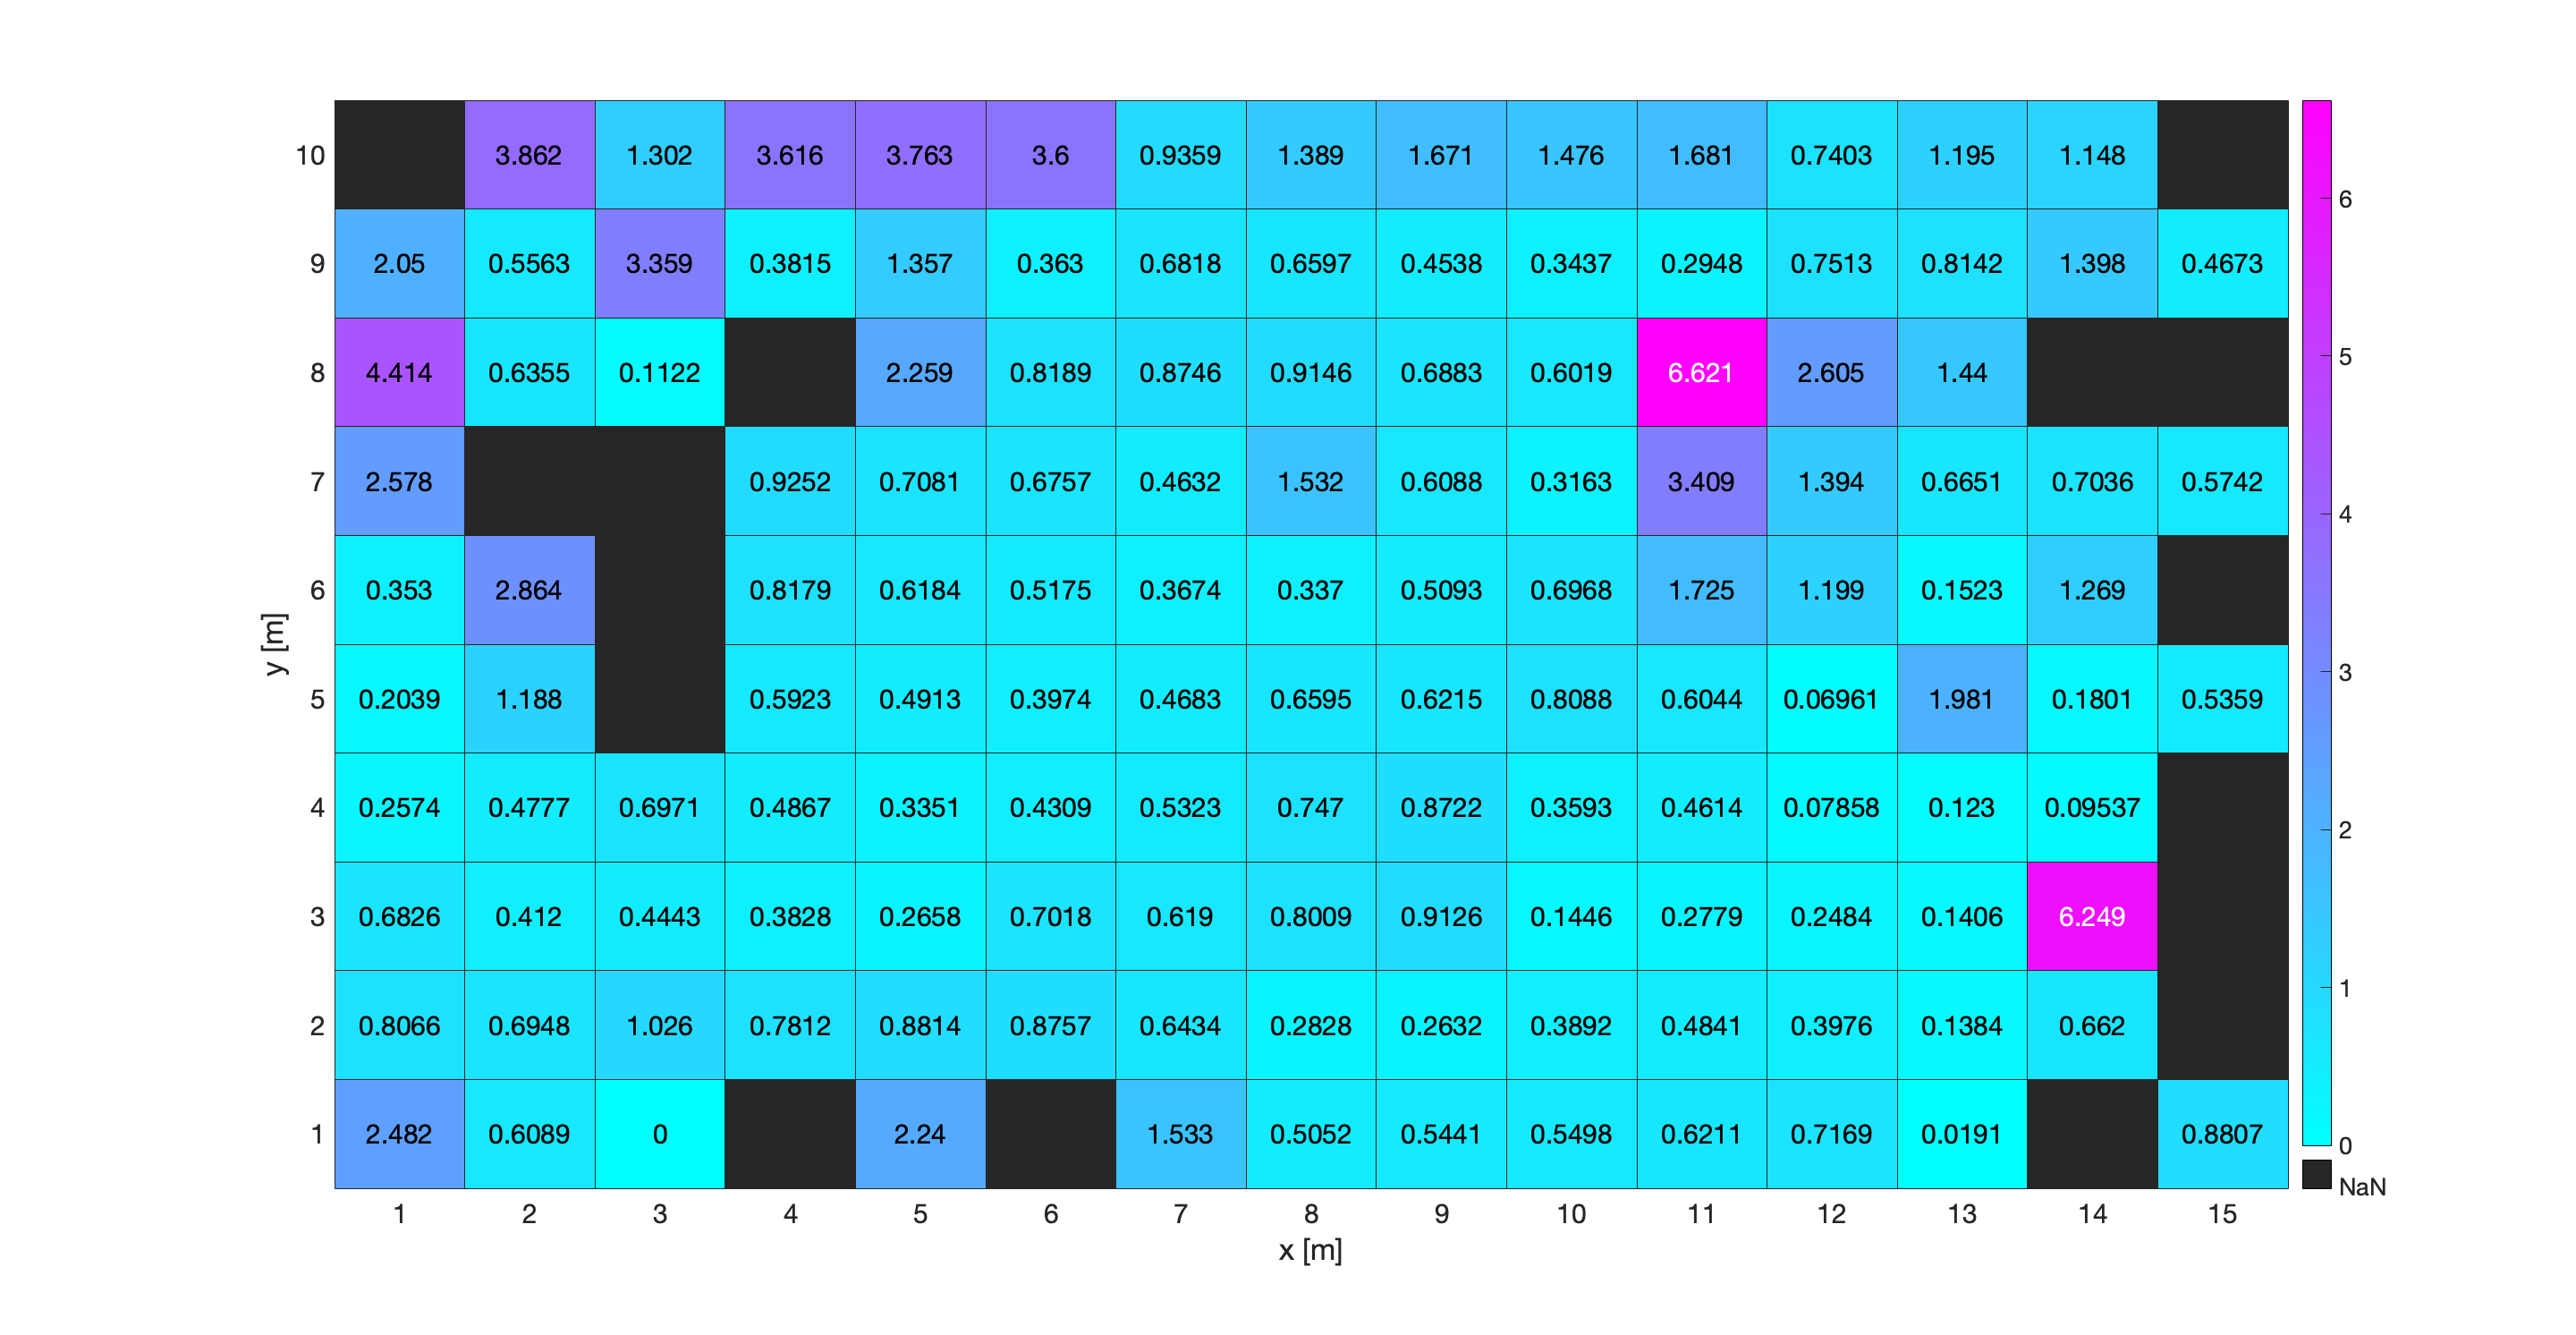
\includegraphics[width=.9\linewidth]{Images/hla_images/hla_anchor_(3_1).png}
\caption{Distance [m] between the tag location and its estimation using the \gls{hla} in an empty room. Anchor being located in (3, 1). \label{fig:hla_empty_1}}
\end{figure}

\begin{figure}[H]
\centering
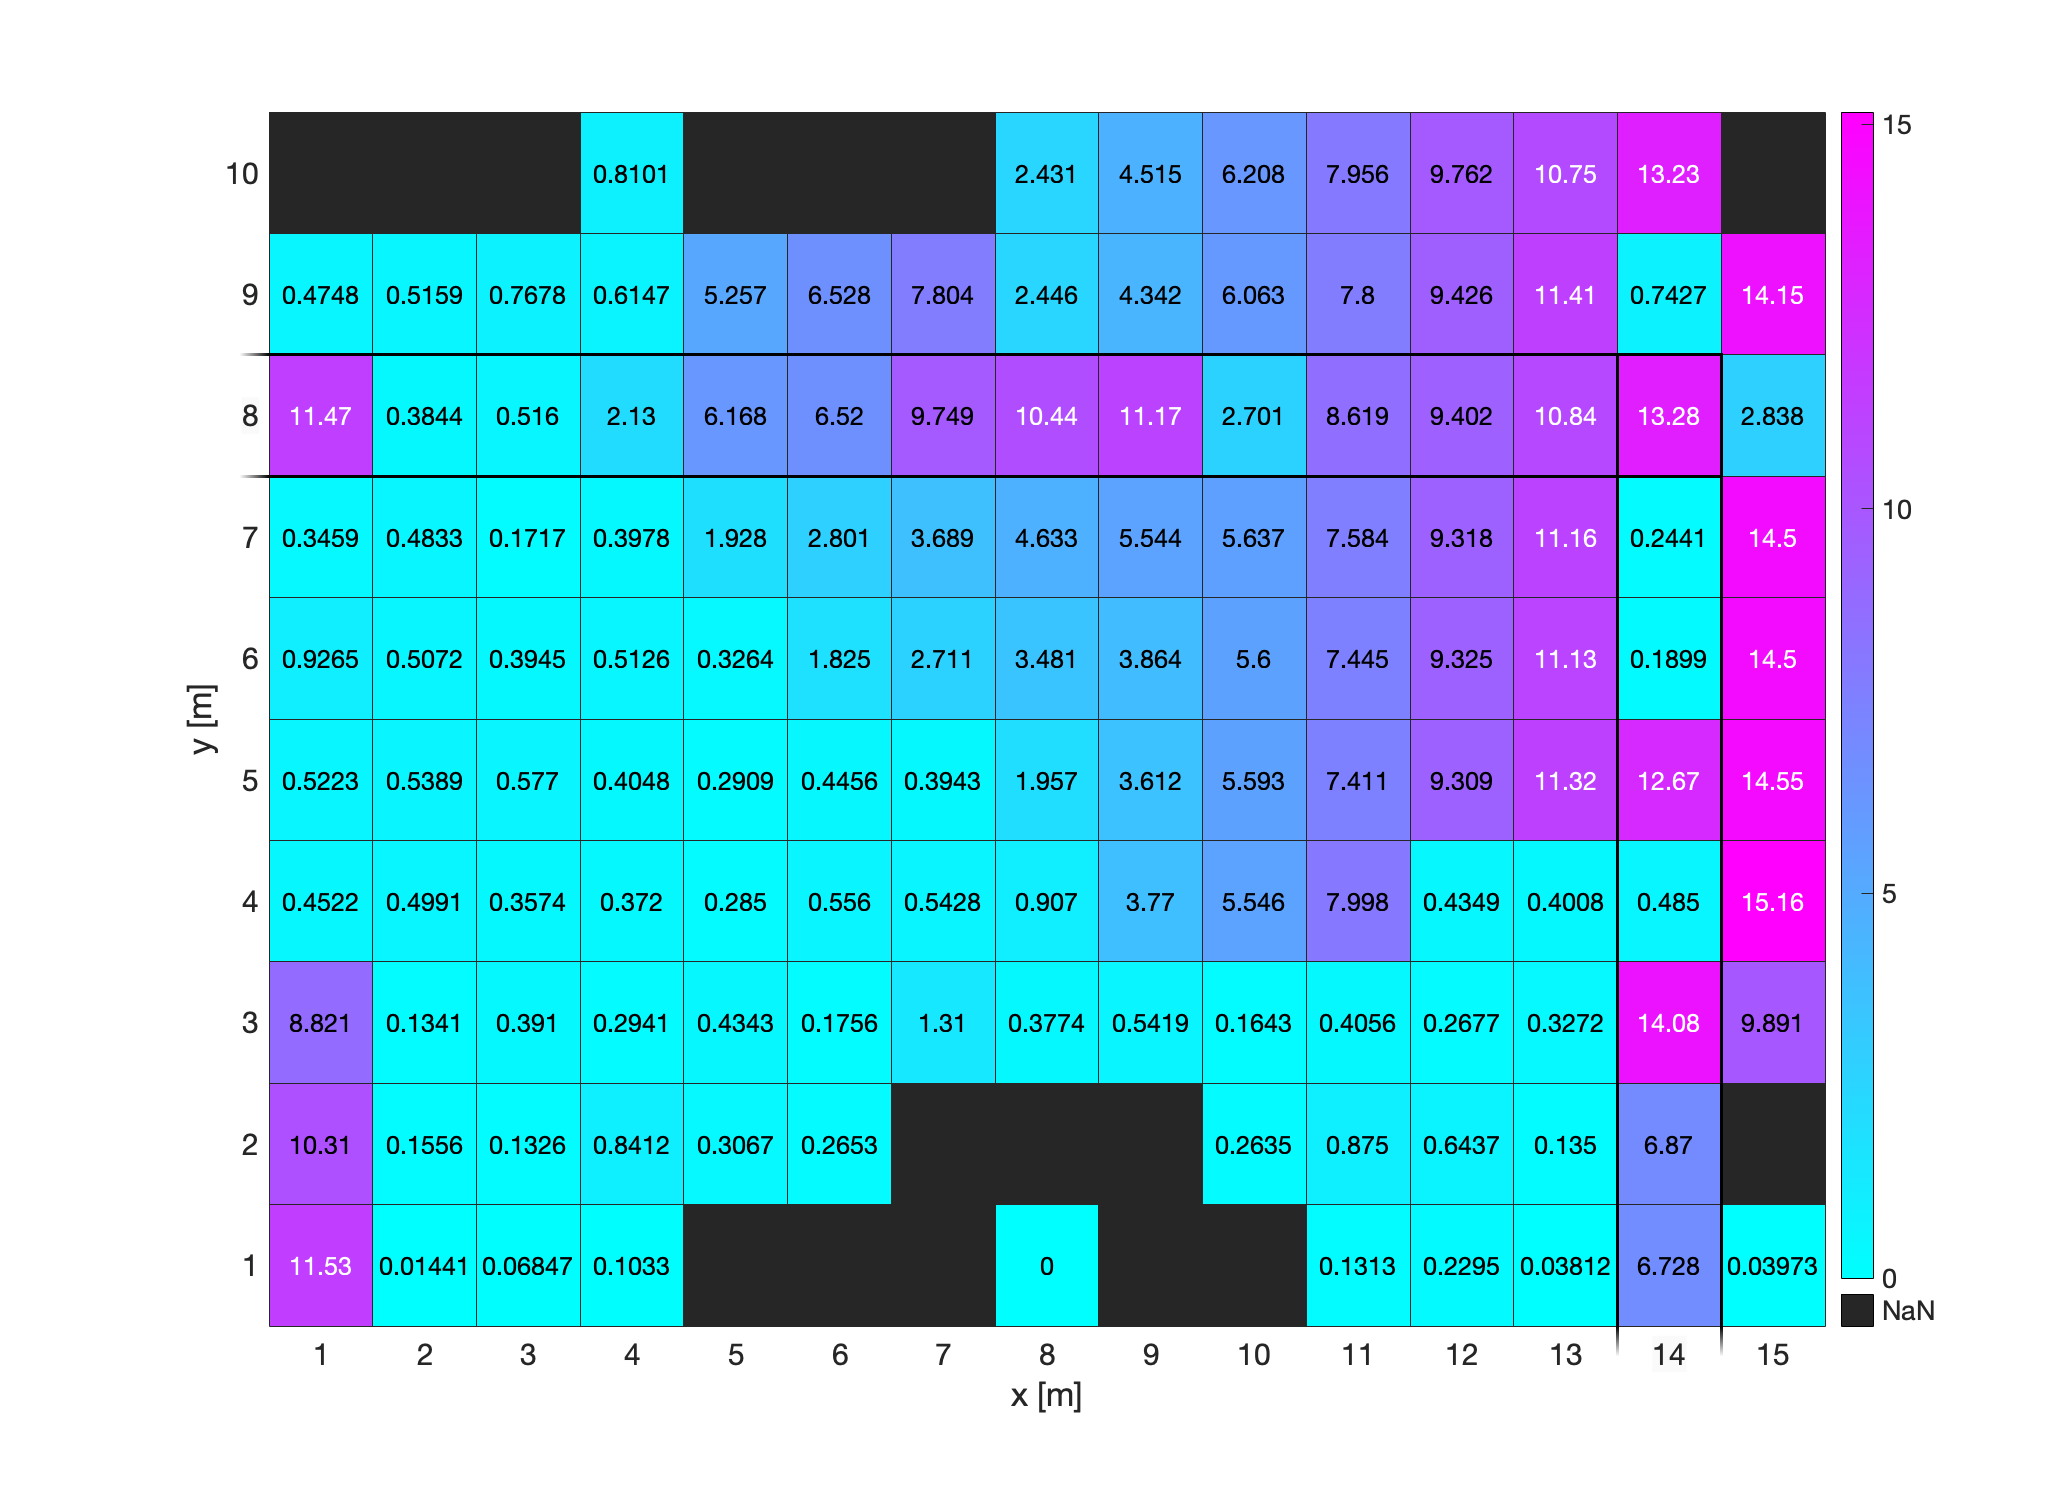
\includegraphics[width=.9\linewidth]{Images/hla_images/anchor_(8_1).png}
\caption{Distance [m] between the tag location and its estimation using the \gls{hla} in an empty room. Anchor being located in (8, 1).\label{fig:hla_empty_2}}
\end{figure}

The top right area of the Fig. \ref{fig:hla_empty_2} shows some rather bad estimations of the tag location. As said, this is most probably due to the symmetry of the room. For most failed estimations from the top right, the \gls{cir} (and so the extracted peaks) of the top right area and its top left counterpart look alike.

\begin{figure}[H]
\centering
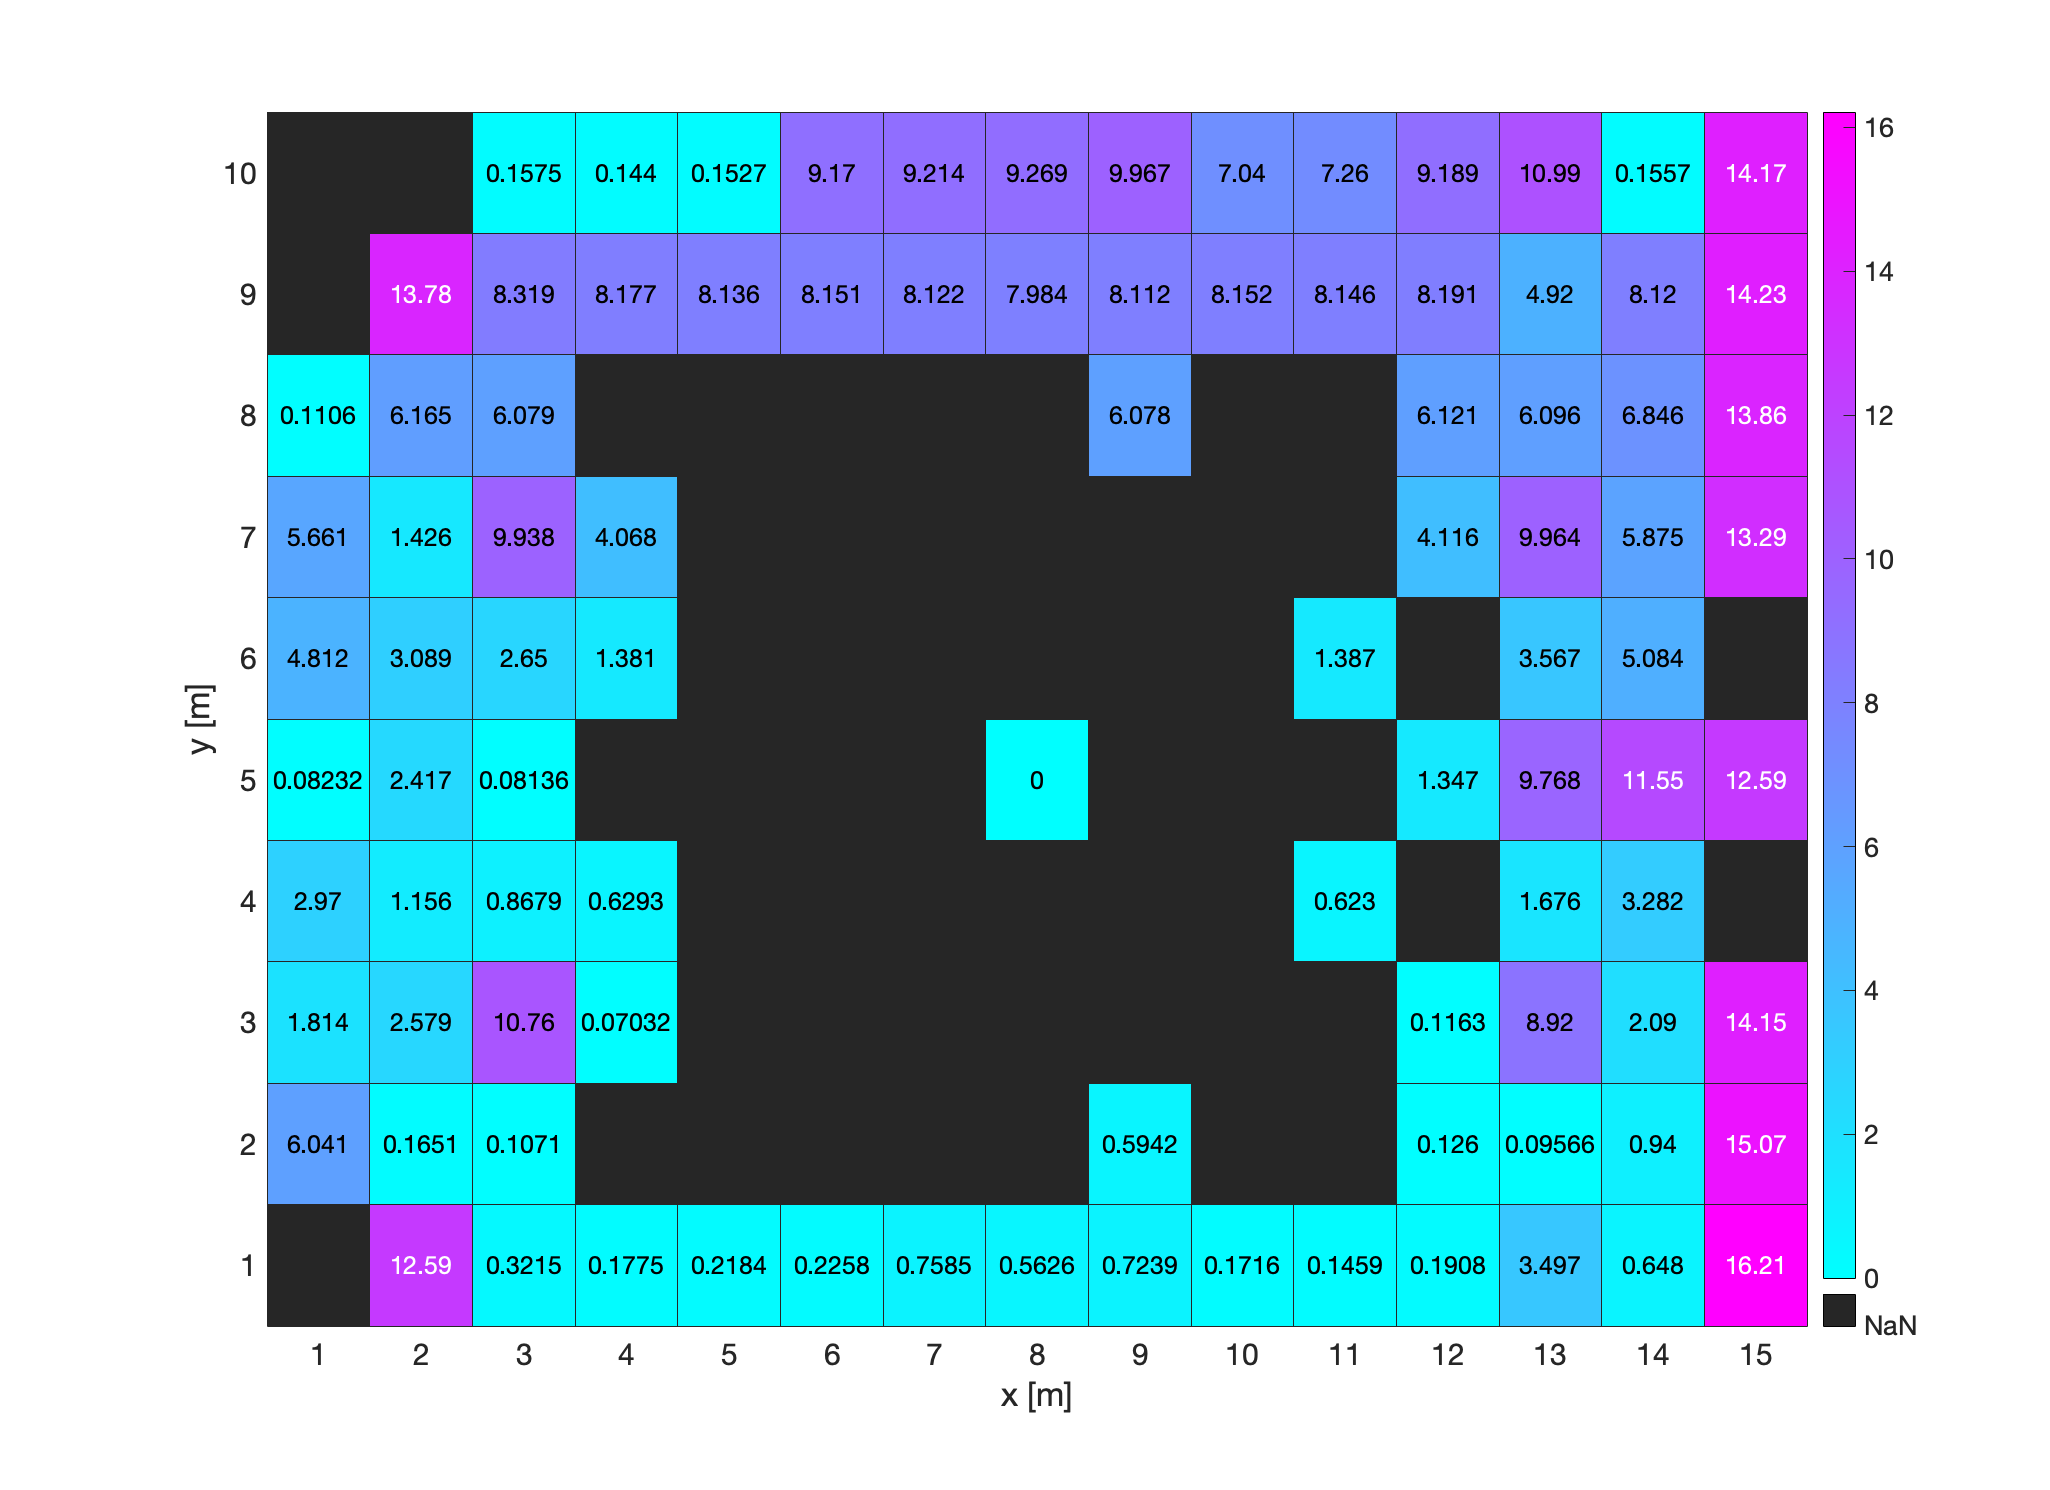
\includegraphics[width=.9\linewidth]{Images/hla_images/anchor_(8_5).png}
\caption{Distance [m] between the tag location and its estimation using the \gls{hla} in an empty room. Anchor being located in (8, 5). \label{fig:hla_empty_3}}
\end{figure}

About Fig. \ref{fig:hla_empty_3}, it is immediate that setting the anchor at the middle of the room is inefficient. This anchor location is located on the intersection of the diagonals and the medians of the room. The same conclusion as for the \gls{sla} algorithm can be made in definitive, the anchor should be located close to a corner to maximize the chances of estimating correctly the exact position of the tag. At least in an empty rectangular room. Next section focuses in some rectangular room filled with furniture.


\subsection{Hard localization in a cluttered room}

In this section, we investigate the room configurations filled with furniture. The two configurations are the same as in section \ref{simu_soft_clut}, the first using the blue furniture only while the second having the blue and green furniture. Some \gls{cir} of places where the localization could not be performed are shown in Fig. \ref{fig:cir_hla_1}, \ref{fig:cir_hla_2}.

\begin{figure}[H]
\centering
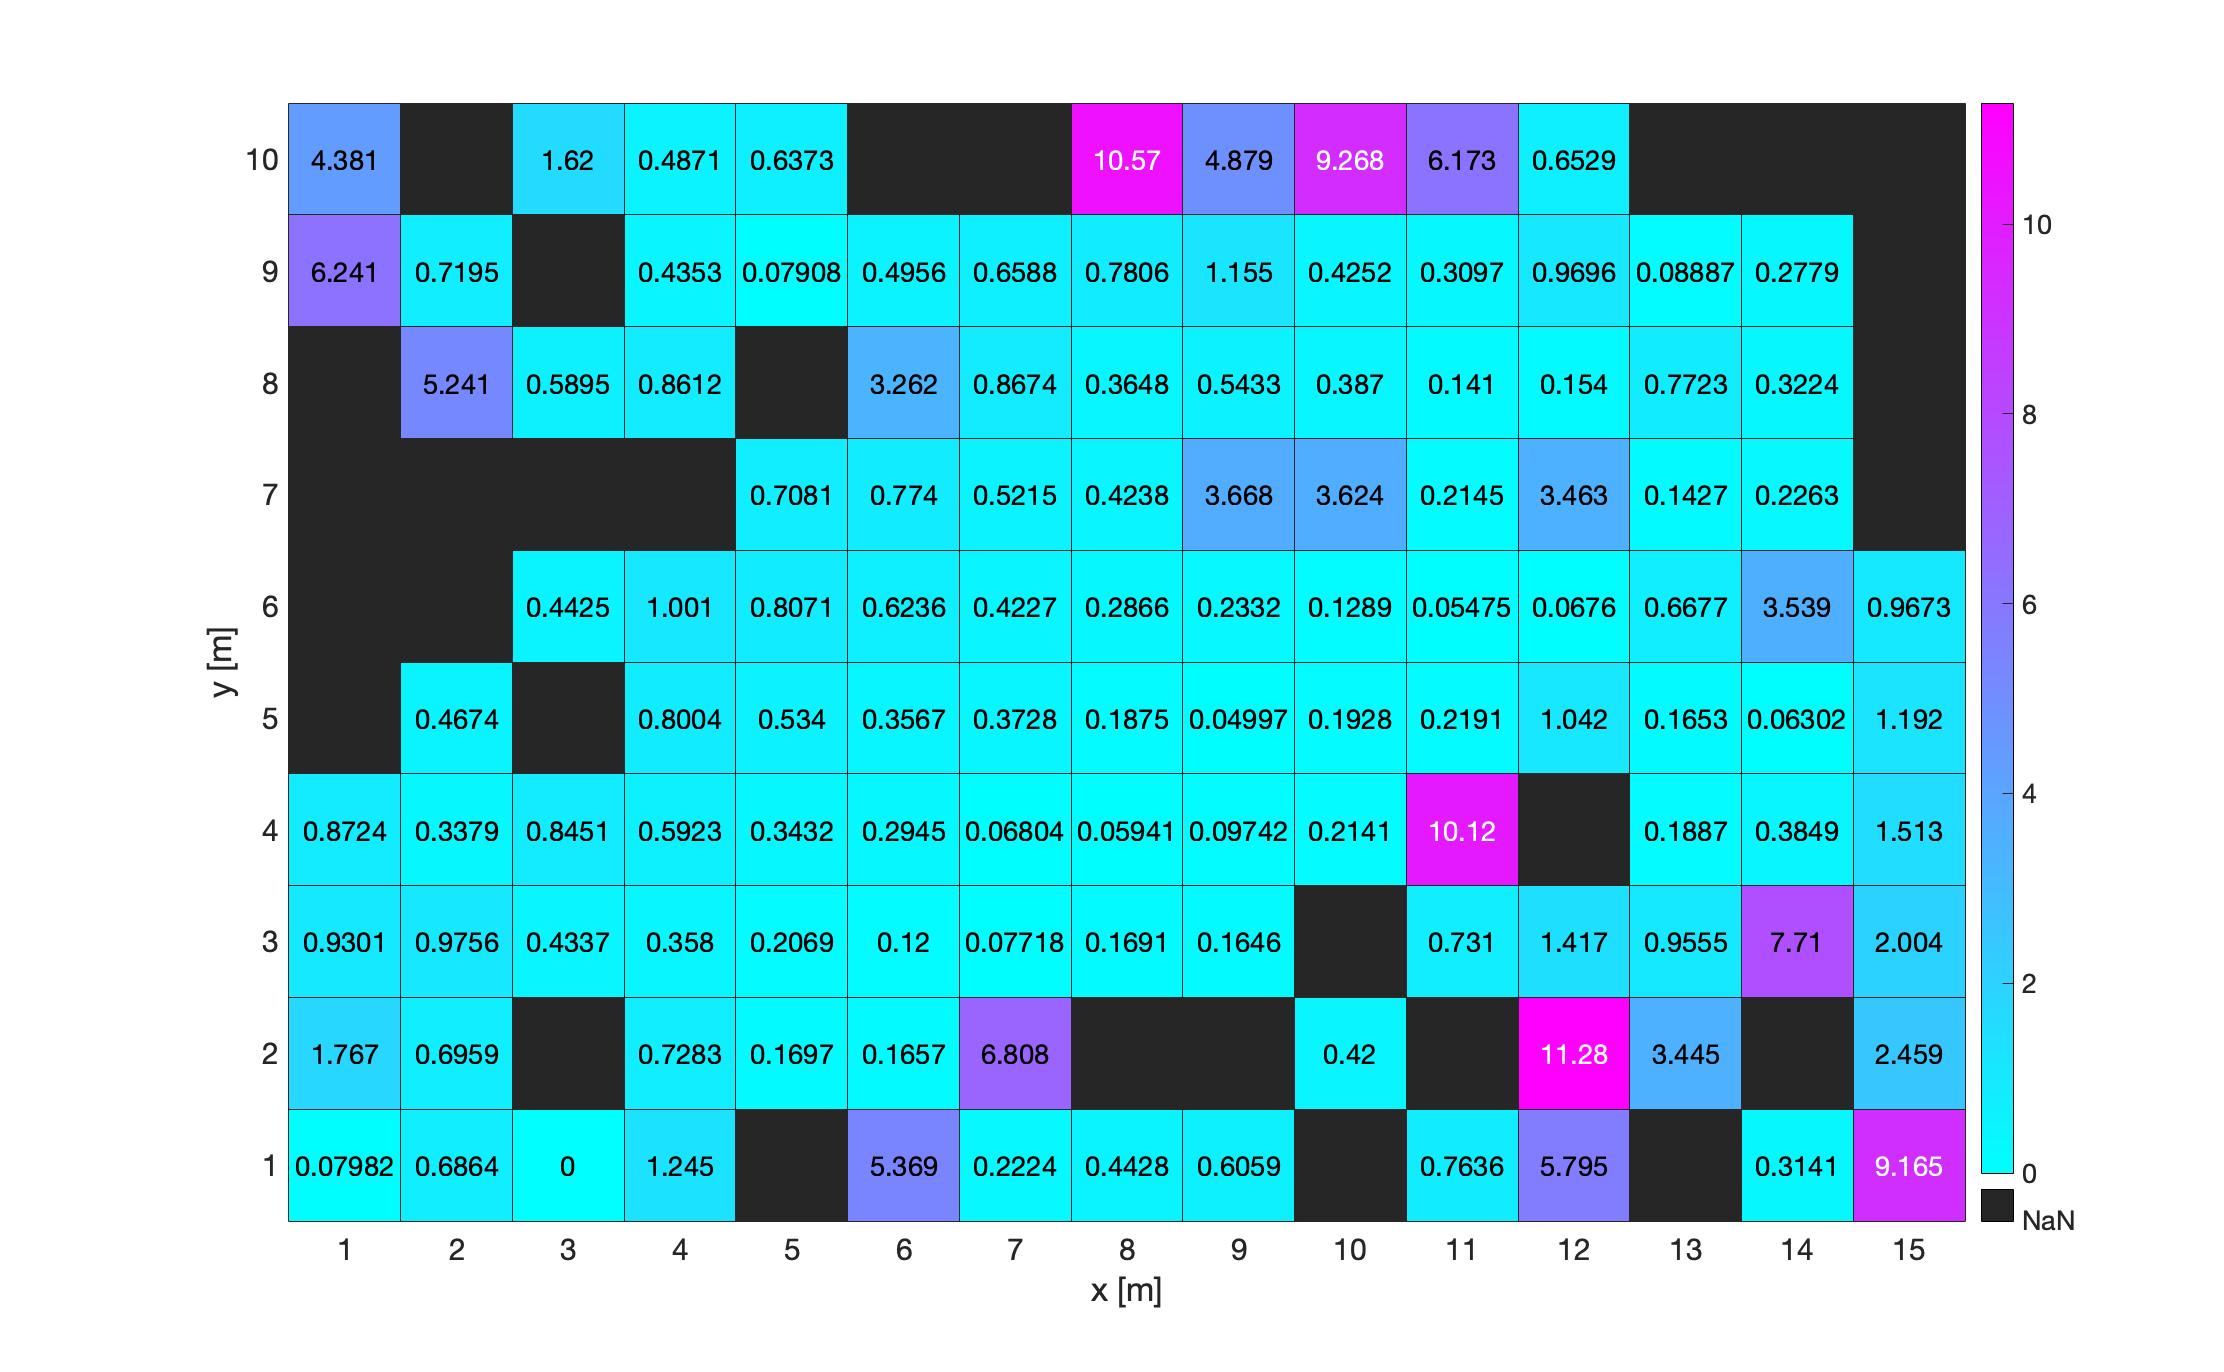
\includegraphics[width=.9\linewidth]{Images/hla_images/anchor_clut_(3_1).png}
\caption{Distance [m] between the real position of the tag and its estimation using the \gls{hla}. The room configuration has only the blue furniture from Fig. \ref{fig:room_cluttered}.\label{fig:hla_little_clut}}
\end{figure}

About the room having less furniture, when comparing to an empty room it appears that the overall precision on the localization decreases. More locations were not estimated at all or were wrongly estimated.

\begin{figure}[H]
\centering
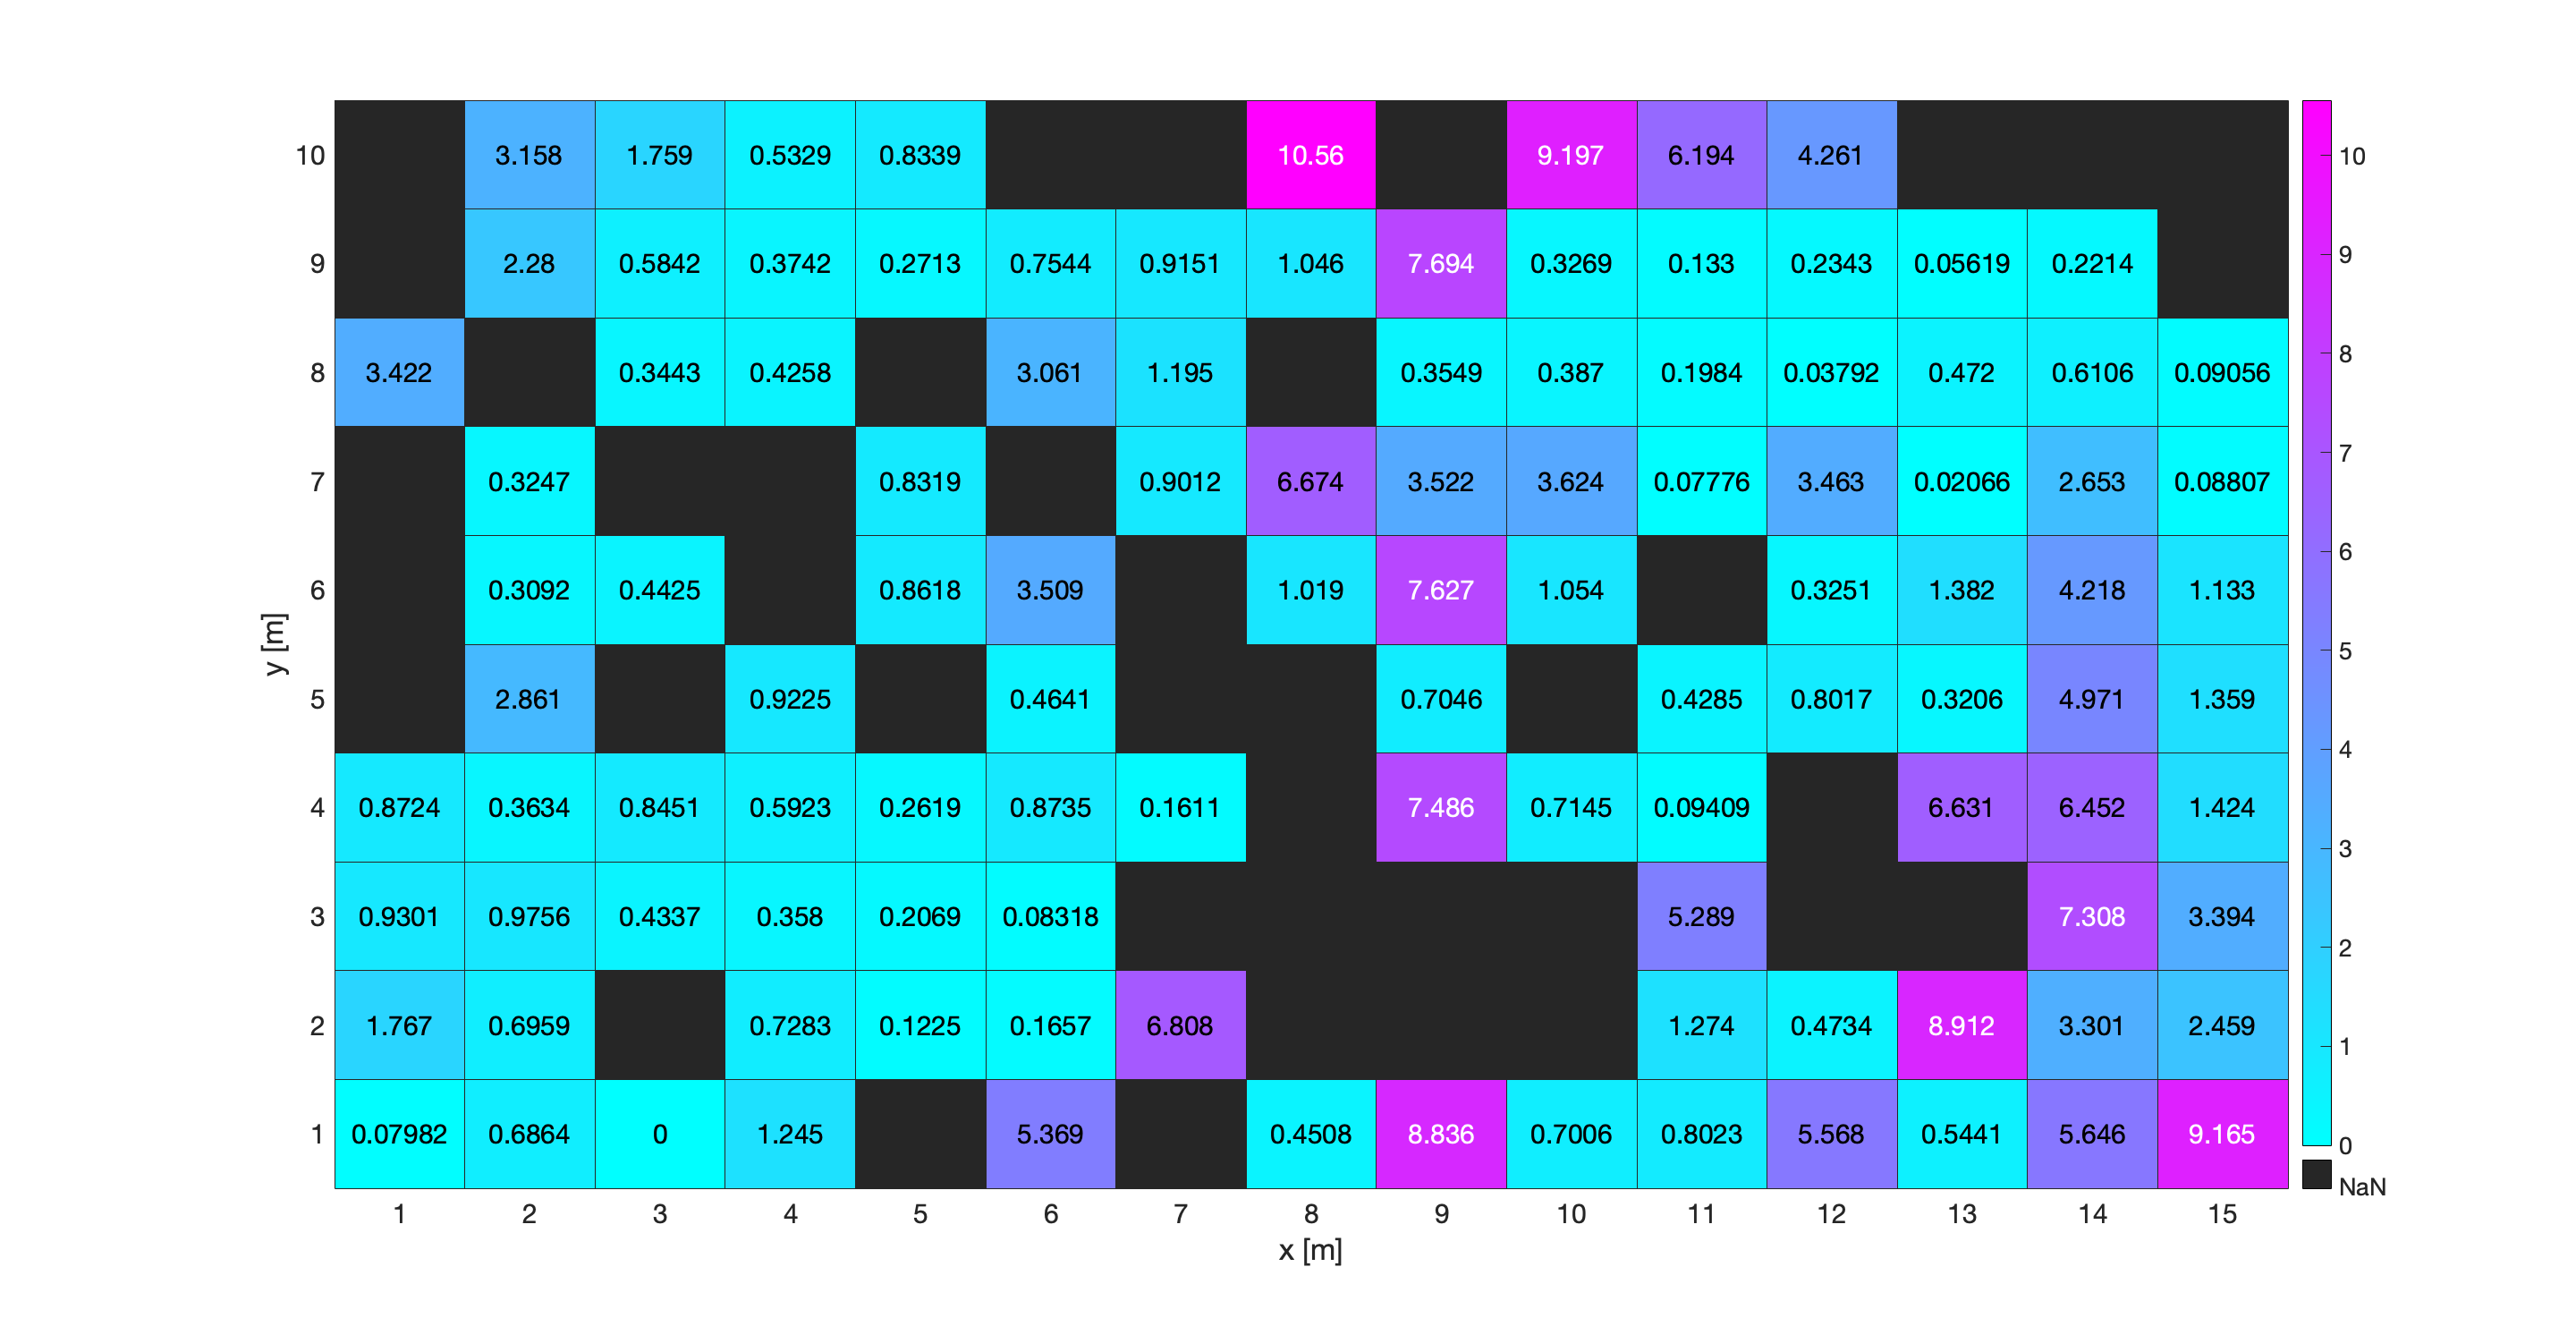
\includegraphics[width=.9\linewidth]{Images/hla_images/really_clut_(3_1).png}
\caption{Distance [m] between the real position of the tag and its estimation using the \gls{hla}. The room configuration has all the furniture from Fig. \ref{fig:room_cluttered}.\label{fig:hla_really_clut}}
\end{figure}

This becomes even worse when including walls in the middle of the room as we can see on Fig. \ref{fig:hla_really_clut}. It appears that location is still possible in part of the room,
as in the \gls{sla} case. But it can not be characterized as reliable.

\begin{figure}[H]
\centering
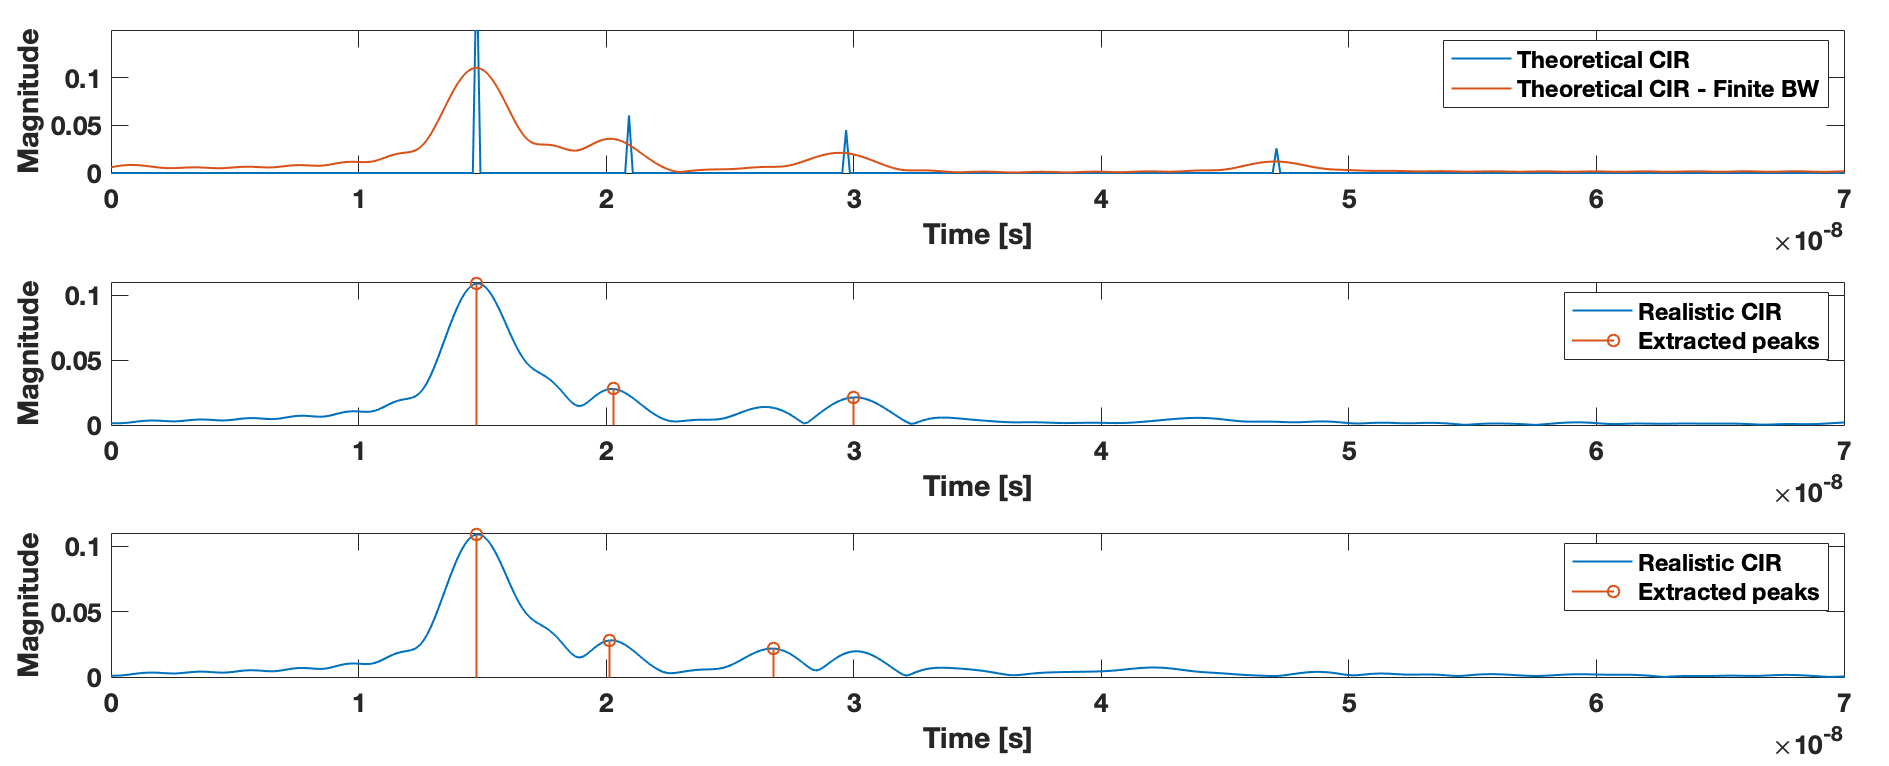
\includegraphics[width=.9\linewidth]{Images/hla_images/image_2.png}
\caption{CIR generated for an anchor located at (3, 1) and a tag at (5, 5) in a room of dimension 15 by 10 m. (Top) Theoretical CIR, direct ray and simple reflections in an empty room. (Middle) Realistic CIR in a room with blue furniture from Fig. \ref{fig:room_cluttered}. (Bottom) Realistic CIR in a room with all the furniture from Fig. \ref{fig:room_cluttered}.. \label{fig:cir_hla_2}}
\end{figure}

In Fig. \ref{fig:cir_hla_1}, the location (5, 5) corresponds to a point which is well localized in the lightly cluttered case but is not localized at all in the heavily cluttered case. This can be understood by looking at the different \gls{cir}. The peaks extracted from the middle \gls{cir} have a good correspondence with the peaks corresponding to the reflected rays in the theoretical \gls{cir}. The bottom \gls{cir} corresponds to a case were no solution was found, indeed, no correspondence can be made between the peaks extracted from the bottom \gls{cir} and the theoretical peaks. Finding another solution which is not the one wished is another possible outcome from such situation.

\begin{figure}[H]
\centering
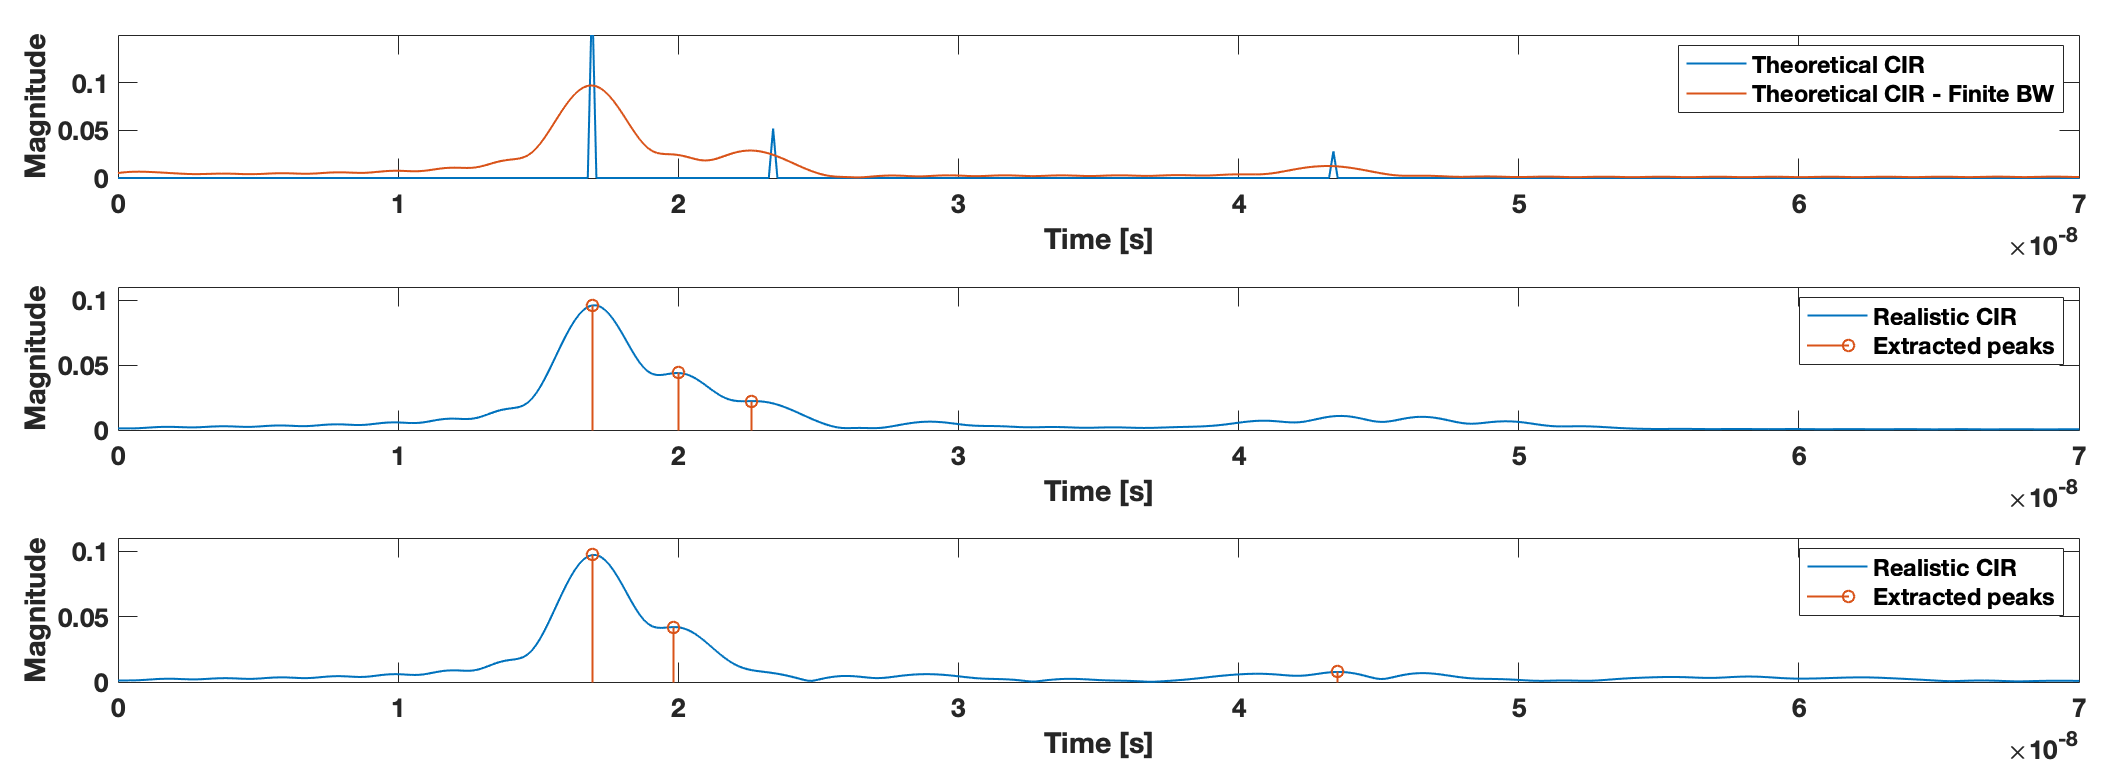
\includegraphics[width=.9\linewidth]{Images/image_1.png}
\caption{CIR generated for an anchor located at (3, 1) and a tag at (2, 6) in a room of dimension 15 by 10 m. (Top) Theoretical CIR, direct ray and simple reflections in an empty room. (Middle) Realistic CIR in a room with blue furniture from Fig. \ref{fig:room_cluttered}. (Bottom) Realistic CIR in a room with all the furniture from Fig. \ref{fig:room_cluttered}. \label{fig:cir_hla_1}}
\end{figure}

In Fig. \ref{fig:cir_hla_1}, the location (2, 6) corresponds to a point which is not localized in the lightly cluttered case but is estimated in the heavily cluttered room. The \glspl{cir} explain this behaviour, but more importantly, this shows that the complex geometry of the room influences completely the \gls{cir} of each location.



\section{Simulations analysis}
\label{simu_anal}

For both algorithms implemented, the symmetry issues were investigated. In both cases, the conclusion was the same, setting the anchor in a corner but not on an axis of symmetry seams to give, in overall, the best results for a rectangular room. Cluttered or not.
\vspace{2mm}

About the performance of both algorithms, it appears to vary in function of the geometry of the room as well as the furniture in it. A lot of variation are simply function of the position of the anchor as it can be seen in the appendices \ref{app:sla}, \ref{app:hla}. Both algorithms can be improved by studying the peak extraction for both cases or more specifically, for the \gls{sla} by including the 'soft' choice for the best estimation or for the \gls{hla} by changing the extracted peaks when no solution is found for the system.


